%%%%%%%%%%%%%%%%%%%%%%%%%%%%%%%%%%%%%%%%%
% Journal Article
% LaTeX Template
% Version 1.3 (9/9/13)
%
% This template has been downloaded from:
% http://www.LaTeXTemplates.com
%
% Original author:
% Frits Wenneker (http://www.howtotex.com)
%
% License:
% CC BY-NC-SA 3.0 (http://creativecommons.org/licenses/by-nc-sa/3.0/)
%
%%%%%%%%%%%%%%%%%%%%%%%%%%%%%%%%%%%%%%%%%

%----------------------------------------------------------------------------------------
%	PACKAGES AND OTHER DOCUMENT CONFIGURATIONS
%----------------------------------------------------------------------------------------

\documentclass[twoside]{article}

\usepackage{lipsum} % Package to generate dummy text throughout this template

\usepackage[sc]{mathpazo} % Use the Palatino font
\usepackage{amsmath}
\usepackage[T1]{fontenc} % Use 8-bit encoding that has 256 glyphs
\linespread{1.05} % Line spacing - Palatino needs more space between lines
\usepackage{microtype} % Slightly tweak font spacing for aesthetics

\usepackage[hmarginratio=1:1,top=32mm,columnsep=20pt]{geometry} % Document margins
\usepackage{multicol} % Used for the two-column layout of the document
\usepackage[hang, small,labelfont=bf,up,textfont=it,up]{caption} % Custom captions under/above floats in tables or figures
\usepackage{booktabs} % Horizontal rules in tables
\usepackage{float} % Required for tables and figures in the multi-column environment - they need to be placed in specific locations with the [H] (e.g. \begin{table}[H])
\usepackage{hyperref} % For hyperlinks in the PDF

\usepackage{lettrine} % The lettrine is the first enlarged letter at the beginning of the text
\usepackage{paralist} % Used for the compactitem environment which makes bullet points with less space between them

\usepackage{abstract} % Allows abstract customization
\renewcommand{\abstractnamefont}{\normalfont\bfseries} % Set the "Abstract" text to bold
\renewcommand{\abstracttextfont}{\normalfont\small\itshape} % Set the abstract itself to small italic text

\usepackage{float}% Places a thin box around figures
\floatstyle{boxed} 
\restylefloat{figure}
\usepackage{graphicx}


\usepackage{titlesec} % Allows customization of titles
\renewcommand\thesection{\Roman{section}} % Roman numerals for the sections
\renewcommand\thesubsection{\Roman{subsection}} % Roman numerals for subsections
\titleformat{\section}[block]{\large\scshape\centering}{\thesection.}{1em}{} % Change the look of the section titles
\titleformat{\subsection}[block]{\large}{\thesubsection.}{1em}{} % Change the look of the section titles

\usepackage{fancyhdr} % Headers and footers
\pagestyle{fancy} % All pages have headers and footers
\fancyhead{} % Blank out the default header
\fancyfoot{} % Blank out the default footer
\fancyhead[C]{Heavy Photon Search Collaboration Note $\bullet$ May 2016} % Custom header text
\fancyfoot[RO,LE]{\thepage} % Custom footer text

%----------------------------------------------------------------------------------------
%	TITLE SECTION
%----------------------------------------------------------------------------------------

\title{\vspace{-15mm}\fontsize{24pt}{10pt}\selectfont\textbf{HPS Ecal Energy Calibration for the Spring 2015 Engineering Run}} % Article title

\author{
\large
\textsc{Holly Szumila-Vance}\\[2mm] % Your name
\normalsize Old Dominion University\\ % Your institution
\normalsize \href{mailto:hszumila@jlab.org}{hszumila@jlab.org} % Your email address
\vspace{-5mm}
}
\date{}

%----------------------------------------------------------------------------------------

\begin{document}

\maketitle % Insert title

\thispagestyle{fancy} % All pages have headers and footers

%----------------------------------------------------------------------------------------
%	ABSTRACT
%----------------------------------------------------------------------------------------

\begin{abstract}

\noindent 
This note describes the energy calibration of the HPS Ecal during the Spring 2015 engineering run. In this calibration, the energy deposition from cosmic ray muons was used to establish initial gains for data acquisition prior to beam running. A more precise energy calibration was achieved by using the energy deposition in each crystal from elastically-scattered electrons carrying the energy of the beam at 1.05 GeV. Sampling fraction correction functions, originally derived from Monte Carlo, were fine-tuned throughout a range of energies by using data from the physics process of Wide-Angle Bremsstrahlung. The culmination of these studies resulted in an improved understanding of the energy resolution that could be used to improve the invariant mass resolution in the search for the Heavy Photon.  
\end{abstract}

%----------------------------------------------------------------------------------------
%	ARTICLE CONTENTS
%----------------------------------------------------------------------------------------

\begin{multicols}{2} % Two-column layout throughout the main article text

\section{Introduction}

%\lettrine[nindent=0em,lines=3]{T} 
The HPS Ecal's primary purpose is for triggering events for read out. Offline, timing is important to the success of HPS as it can be used to reduce accidentals in two-cluster events and improve cluster reconstruction. The two-cluster pairs trigger is the primary trigger used by HPS in order to find correlated $e^+e^-$ events for reconstructing the invariant mass and analyzing the invariant mass spectrum for a possible Heavy Photon signal.\\ 
\indent The PbWO$_4$ crystals of the Ecal are readout using FADC250s which sample the input signals at 250 MHz, or every 4 ns. All data taken during the Spring 2015 running was taken using the FADC250 Mode 1 which corresponds to the full raw waveform read out. In offline reconstruction, each pulse is fit using a 3-pole function that is detailed in ~\cite{Baltzell}. The time for a hit is obtained from the parameters in this fitting method. Clusters are formed by searching for seed hits (highest energy crystal with all surrounding crystals lower in energy) and adding hits that surround the seed hits. Clustering can be improved with detailed studies of timing so that out of time hits from different events are not added to clusters. 
\indent For precision time measurement, the crystals were calibrated using the accelerator RF signal which enters Hall B at 499 MHz and is sampled every 80 signals ~\cite{Kazimi}. The RF signal is  split in the hall and readout by two FADC250 channels.

%------------------------------------------------
\section{Simulations}

Simulations were performed in SLIC using the HPS-EngRun-2015-Nominal-v3 geometry which uses surveyed values for the detector positions in Hall B as well as the corresponding magnetic field setting used in 1 GeV running. The procedure for the simulations is similar to what is described in Ref ~\cite{Garcon}.\\
\indent Single particles: electrons, positrons, and photons were simulated at discrete energies of 0.2, 0.3, 0.4, 0.5, 0.6, 0.7, 0.8, 0.9, 1.0, and 1.1 GeV in order to uniformly cover the range of energies detectable in the spring 2015 running at 1.05 GeV. The simulation fully utilizes the procedures for HPS Monte Carlo reconstruction which differs slightly from the individual hit readout methods used in Ref ~\cite{Garcon}. The offline cluster reconstruction uses the same thresholds used in data and production Monte Carlo: 7.5 MeV for individual hits, 50 MeV for seed hits in clusters, 100 MeV for cluster energies. The sampling fraction correction function for electrons is shown in Figure ~\ref{mcsf_em}.  

\begin{figure}[H]
  \centering
      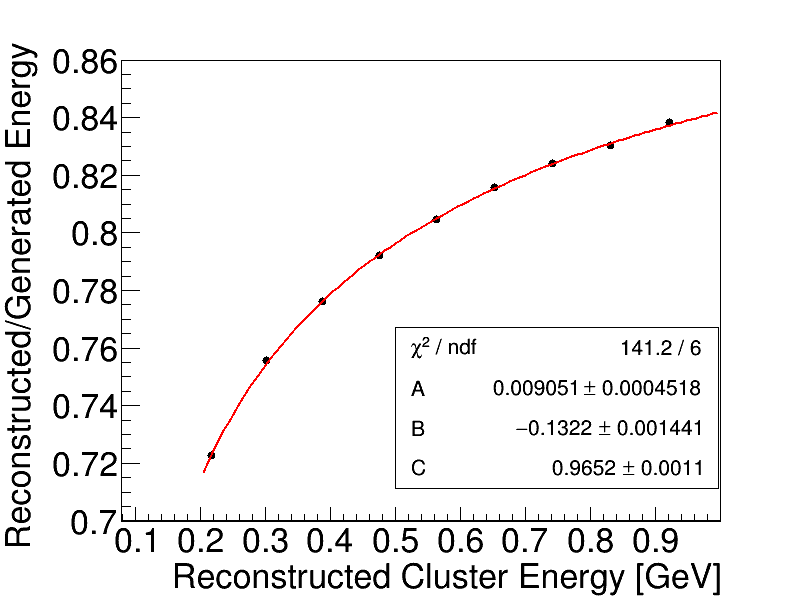
\includegraphics[width=0.5\textwidth]{pics/fidSF_em.png}
  \caption{Electron sampling fraction as found in Monte Carlo with a fiducial cut.}
  \label{mcsf_em}
\end{figure}	

In general, the clusters for all three types of particles with a simulated energy $>$ 200~MeV have been reliably reconstructed. The form of the sampling fraction correction function, as described in Ref ~\cite{Garcon}, is a three parameter fit:

\begin{equation}
\label{eq:samplingfraction}
\dfrac{E_{rec}}{E_{gen}} = \dfrac{A}{E_{rec}}+\dfrac{B}{\sqrt{E_{rec}}}+C 
\end{equation}	

In Equation ~\ref{eq:samplingfraction}, the subscript $rec$ refers to the reconstructed energy (clustering applied to energy deposited in the Ecal), whereas the subscript $gen$ refers to the generated Monte Carlo energy which corresponds to the energy carried by the particle that deposits its energy into the Ecal. The sampling fractions described by these Monte Carlo simulations versus the ones found previously ~\cite{Garcon} differ due to more precise Monte Carlo modeling of hit reconstruction of the energy deposited within a PbWO$_4$ crystal and utilize a slightly shifted geometry with a lower magnetic field that corresponds to 1.1 GeV running. The updated sampling fraction correction functions for positrons and photons, as found in Monte Carlo, are shown in Figures ~\ref{mcsf_ep} and ~\ref{mcsf_p}, respectively.   
 
\begin{figure}[H]
  \centering
      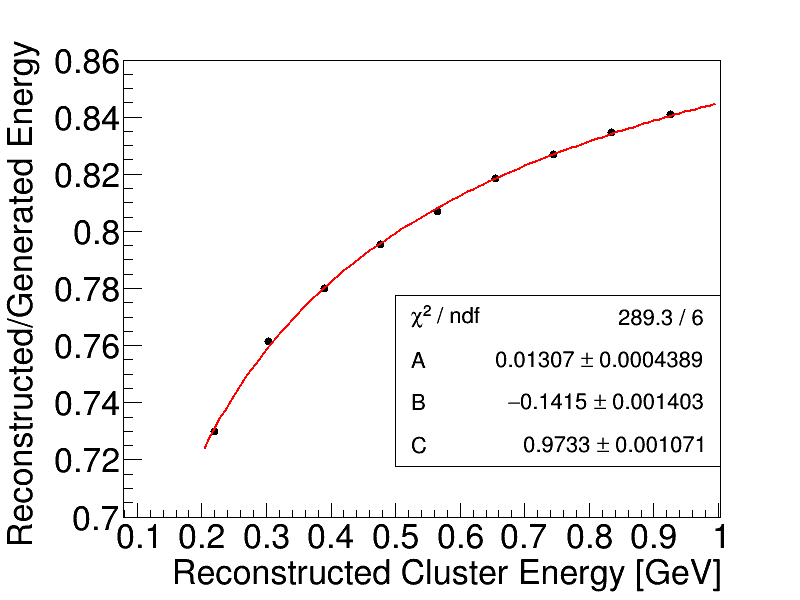
\includegraphics[width=0.5\textwidth]{pics/fidSF_ep.png}
  \caption{Positron sampling fraction as found in Monte Carlo with a fiducial cut.}
  \label{mcsf_ep}
\end{figure}


\begin{figure}[H]
  \centering
      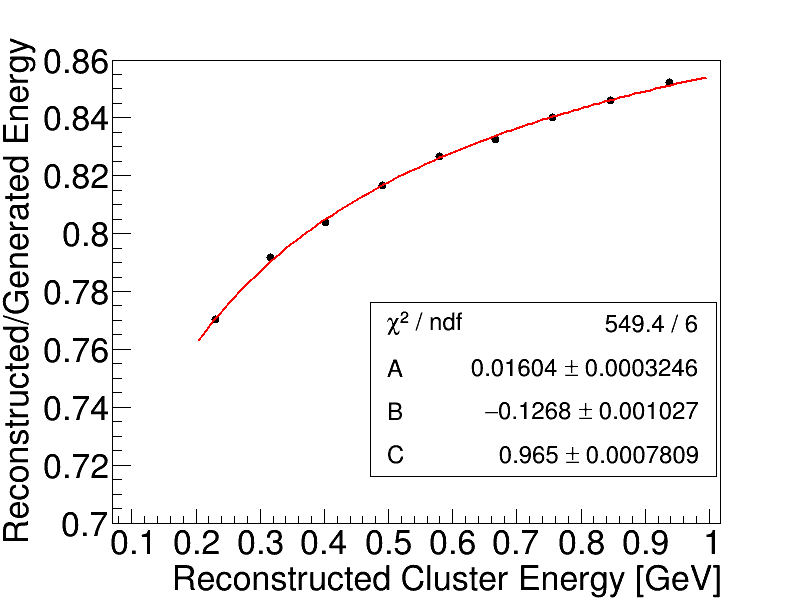
\includegraphics[width=0.5\textwidth]{pics/fidSF_p.png}
  \caption{Photon sampling fraction as found in Monte Carlo with a fiducial cut.}
  \label{mcsf_p}
\end{figure} 

The sampling fraction corrections vary for different particle types due to the magnetic field curving positrons and electrons (and the non curvature of photon trajectories) of different energies such that the impact angle of the particles entering the crystals of the calorimeter varies across the calorimeter with position.\\
The energy resolution of the calorimeter in the updated Monte Carlo reconstruction was unchanged from the previous simulation studies in Ref ~\cite{Garcon}. The new Monte Carlo did provide an opportunity to explore the energy leakage effects in the edge crystals of the Ecal in greater detail. The energy leakage effects in the Ecal are parameterized as a function of distance to the innermost edge of the crystals along the beam gap. The energy leakage deteriorates rapidly in the crystal closest to the beam gap, but stabilizes in the central region of the Ecal before dropping off rapidly in the outermost (layer +5 across the top and layer -5 across the bottom) crystals in the Ecal. We can optimally study the sampling fraction for a particular particle as a function of distance to the innermost edge of the Ecal at the beam gap. In Equation ~\ref{eq:samplingfraction}, parameter $A$ is not well-correlated with position and remains as a constant for a given particle type. The parameters $B$ and $C$ are strongly correlated with the position of the cluster relative to the edge of the Ecal. For electrons, we can observe the parameter $B$ as a function of its position relative to the innermost beam gap edge in Figure ~\ref{p1_em}. The Monte Carlo truth information is used to determine the position of the particle at the face of the Ecal whereas in data, this position value will come from SVT tracking information. 

\begin{figure}[H]
  \centering
      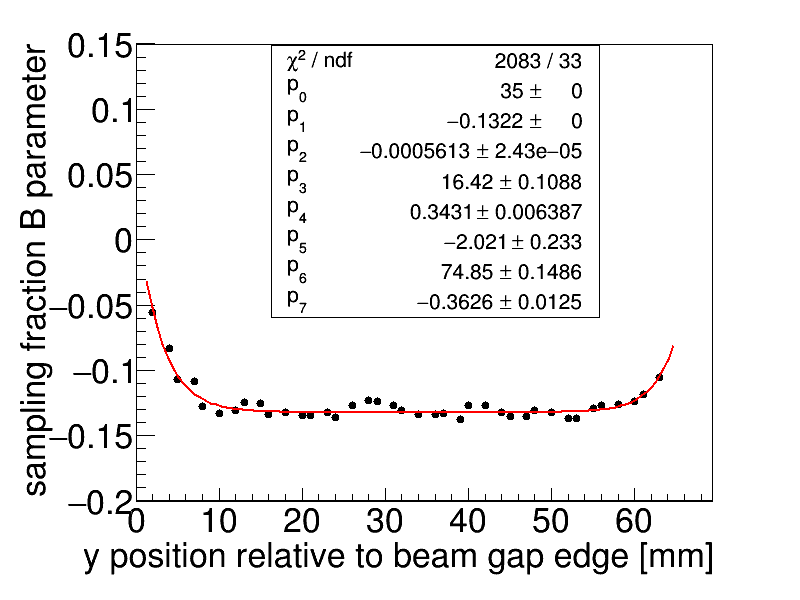
\includegraphics[width=0.5\textwidth]{pics/par0_em.png}
  \caption{Electron sampling fraction parameter, $B$, as a function of position relative to the innermost beam gap edge.}
  \label{p1_em}
\end{figure} 

As shown in Figure ~\ref{p1_em}, the sampling fraction parameter $B$ can be fit with two functions at the edges that match in the central region of the Ecal, away from the edges of the calorimeter. The equations used to fit the $B$ and $C$ sampling fraction parameters are described by Equations ~\eqref{eq:p1parlt} and ~\eqref{eq:p2parlt}.

\begin{equation}
\begin{split}
\label{eq:p1parlt}
B(y<p_0) = p_1-p_2 e^{-(y-p_3)p_4}\\
B(y>p_0) = p_1-p_5 e^{-(y-p_6)p_7}
\end{split}
\end{equation}

\begin{equation}
\begin{split}
\label{eq:p2parlt}
C(y<p_0) = p_1-p_2 e^{-(y-p_3)p_4}\\
C(y>p_0) = p_1-p_5 e^{-(y-p_6)p_7}
\end{split}
\end{equation}

As shown in Equations ~\eqref{eq:p1parlt} and ~\eqref{eq:p2parlt}, the sampling fraction is relatively stable in the central region of the calorimeter and is matched from both the top and bottom edges of the calorimeter at $p_0$. The parameters describing the energy leakage change rapidly in edge crystals. For columns containing 5 crystals, vertically, in each half of the Ecal, the distance to the beam gap edge of the calorimeter is straight forward. However, for crystals above and below the region of the Ecal where row 1 crystals are removed, additional consideration must be made when calculating the distance to the edge in order to be consistent with the other region of the Ecal.

 Due to the matching of the sampling fraction correction function and parameters at the central region of the Ecal, when immediately above or below the row 1 cutout region, one takes the distance to the bottom edge of the row +/-2 crystals. If above/below the row $\pm$1 cutout region and at a greater distance than the matching point, $p_0$, then the distance is taken to the bottom edge of the row 1 crystals. For any other region with row $\pm$1 crystals, the distance is take to the innermost edge of the row $\pm$1 crystals. These regions and vertical positions in y are shown in Figure ~\ref{ecalY}:

\begin{figure}[H]
  \centering
      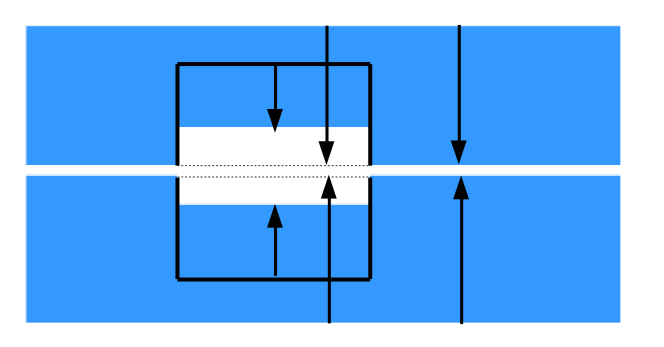
\includegraphics[width=0.5\textwidth]{pics/ecaldistance.png}
  \caption{The Ecal, as viewed from downstream and looking upstream, is shown with arrows to indicate to which location the beam gap edge of the Ecal is being used for calculating the relative position in y. As shown, the region above and below the electron hole are calculated to the edge of the row 2 crystals unless above the region where the matching of the two edge functions occurs.}
  \label{ecalY}
\end{figure}  
\indent The changing parameters of the sampling fraction correction functions can be understood as a function of this position to the beam gap edge of the crystal. As mentioned previously, $B$ and $C$ are strongly correlated with this distance to the edge of the calorimeter. For electrons, the relationship of these parameters with position can be seen in Figures ~\ref{p1_em} and ~\ref{p2_em}.

\begin{figure}[H]
  \centering
      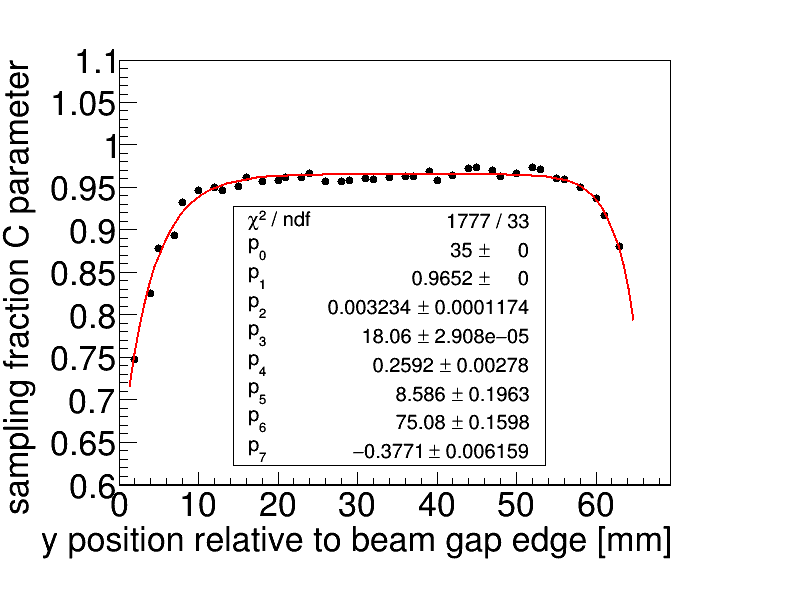
\includegraphics[width=0.5\textwidth]{pics/par1_em.png}
  \caption{Electron sampling fraction parameter, $C$, as a function of position relative to the innermost beam gap edge.}
  \label{p2_em}
\end{figure} 

In Figures ~\ref{p1_em} and ~\ref{p2_em}, all fit parameters shown are consistent with Equations ~\eqref{eq:p1parlt} and ~\eqref{eq:p2parlt}. Thus, it can be observed that all parameters of the sampling fraction correction function match in the fiducial (central) region of the Ecal. The same relationship can be observed by the parameters describing the sampling fraction correction for positrons in Figures ~\ref{p1_ep} and ~\ref{p2_ep}.

\begin{figure}[H]
  \centering
      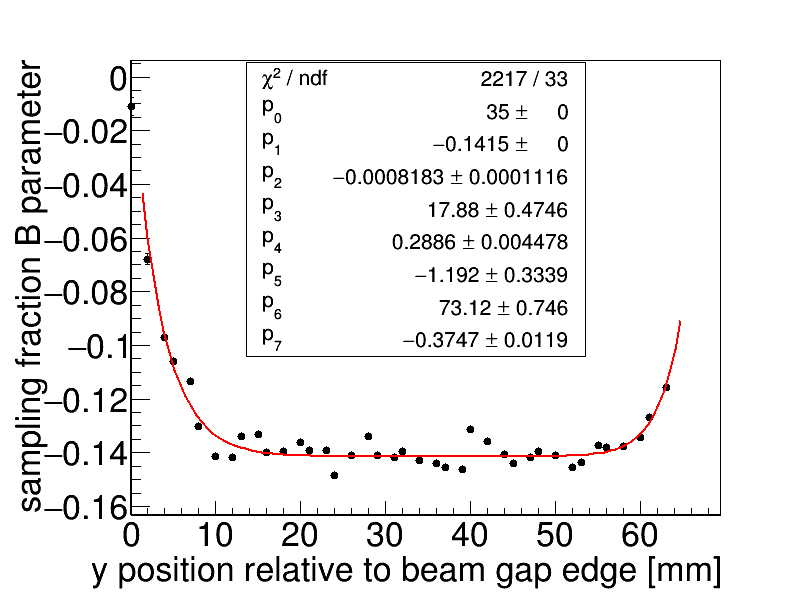
\includegraphics[width=0.5\textwidth]{pics/p0_ep.png}
  \caption{Positron sampling fraction parameter, $B$, as a function of position relative to the innermost beam gap edge.}
  \label{p1_ep}
\end{figure} 

\begin{figure}[H]
  \centering
      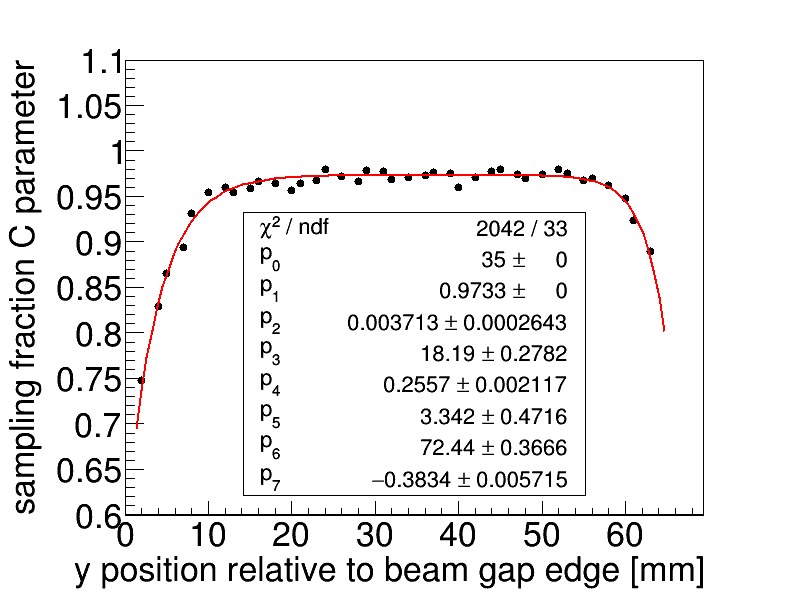
\includegraphics[width=0.5\textwidth]{pics/p1_ep.png}
  \caption{Positron sampling fraction parameter, $C$, as a function of position relative to the innermost beam gap edge.}
  \label{p2_ep}
\end{figure} 

The sampling fraction parameters for photons can also be parameterized in terms of the position from the beam gap edge as shown in Figures ~\ref{p1_p} and ~\ref{p2_p}. While the position used in Monte Carlo comes from knowing the particle's truth information, the position in data will come from the calculated cluster position which can not be calculated past 6.5~mm (halfway) from the edge of the edge crystal. 

\begin{figure}[H]
  \centering
      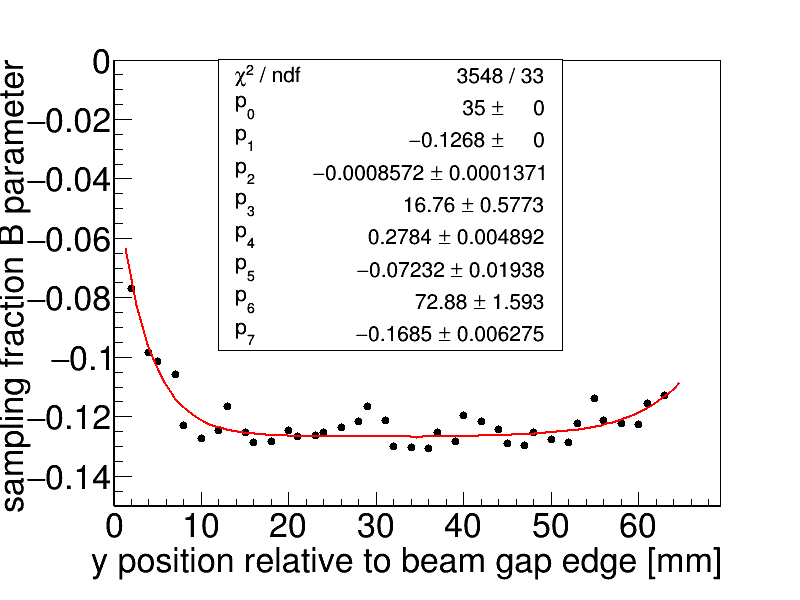
\includegraphics[width=0.5\textwidth]{pics/p0_p.png}
  \caption{Photon sampling fraction parameter, $B$, as a function of position relative to the innermost beam gap edge.}
  \label{p1_p}
\end{figure} 

\begin{figure}[H]
  \centering
      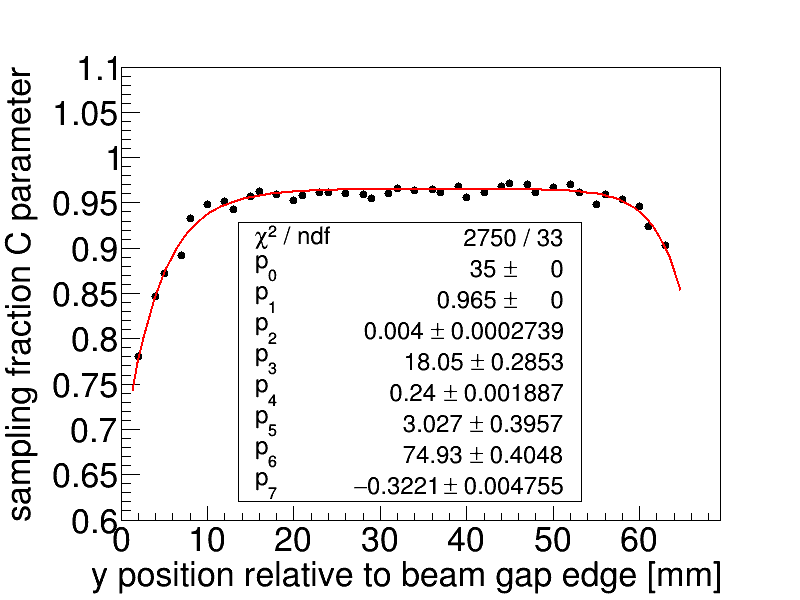
\includegraphics[width=0.5\textwidth]{pics/p1_p.png}
  \caption{Photon sampling fraction parameter, $C$, as a function of position relative to the innermost beam gap edge.}
  \label{p2_p}
\end{figure} 

The simulations are critical for understanding the energy leakage in the edge crystals of the calorimeter. While the general fiducial sampling fraction can be studied with data, the full energy correction at the edges is difficult to derive empirically as the energy resolution deteriorates substantially.



\section{Energy Calibration}

The Ecal was calibrated both in energy and time. An initial energy calibration was conducted prior to any electron beam on target by using the energy deposition from cosmic ray muons. The timing calibration was accomplished with data collected during beam running and used the accelerator RF signal ~\cite{Szumila}. The final energy calibration utilized physics events from elastic scattering and wide angle bremsstrahlung collected during experimental beam running.  \\
\indent Prior to the first experimental running in the fall of 2014, each crystal of the Ecal was upgraded with large area Avalanche Photo Diodes (APDs) for readout. APDs collect the photons at the back of each crystal (the number of photons is proportional to the energy deposited by a particle into the crystal) and convert this measurement into an electronic signal. The large area Hamamatsu S8664-3189 APDs enabled the Ecal to have the sensitivity to detect the tiny signals from cosmic muons traversing the Ecal crystals perpendicularly and then to use this signal for the initial calibration of the modules. 
%%%%%%%%%%%%%%%%%%%%%%%%%%%%%%%%%%%%%%%%%%%%%%%%%%%%%%%%%%%%%%%%%%%%%%%%%%%%%%%%%%%%%%
%\begin{figure}[H]
%  \centering
%      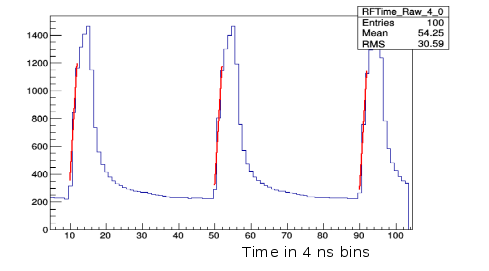
\includegraphics[width=0.5\textwidth]{rfFitting.png}
%  \caption{Straight line fit to the leading edge of the RF signal.}
%  \label{rfsignal}
%\end{figure}	
%%%%%%%%%%%%%%%%%%%%%%%%%%%%%%%%%%%%%%%%%%%%%%%%%%%%%%%%%%%%%%%%%%%%%%%%%%%%%%%%%%%

\subsubsection{Cosmics}

The experimental setup for the cosmic calibrations utilized two scintillators placed below the Ecal to trigger readout of all of the crystals. The setup is shown in Figure ~\ref{cosmicSetup}.

\begin{figure}[H]
  \centering
      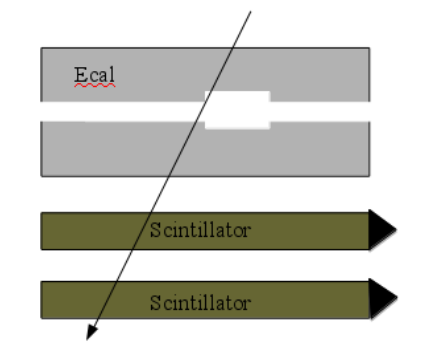
\includegraphics[width=0.5\textwidth]{pics/cosmicsetup.png}
  \caption{Experimental setup for the cosmic ray calibration. As a cosmic ray passes vertically through both scintillators, event readout is triggered.}
  \label{cosmicSetup}
\end{figure}


The experimental setup was modeled using Monte Carlo simulations so that the energy deposited in the crystals from cosmic ray muons and rates could be studied. By measuring the average path length of cosmic ray muons in each crystal, the energy deposited in each crystal of the Ecal was calculated using the known energy deposition from 2~GeV muons ~\cite{pdg}. The average energy per crystal from this calculation was determined to be 18.3~MeV and the variation is seen in Figure ~\ref{cosmicEdep}.

\begin{figure}[H]
  \centering
      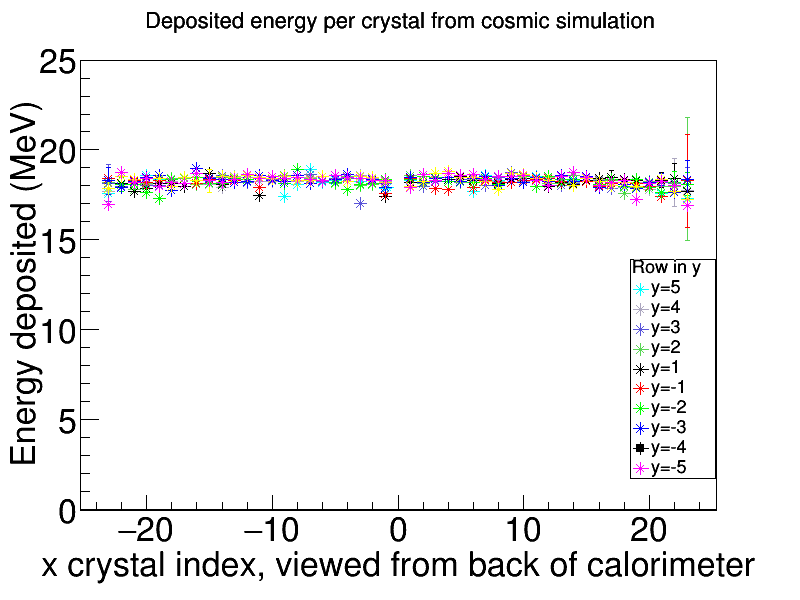
\includegraphics[width=0.5\textwidth]{pics/cosmicEdep.png}
  \caption{The simulated cosmic ray muon energy deposition per crystal of the Ecal. The mean was 18.3 MeV.}
  \label{cosmicEdep}
\end{figure}

In Figure ~\ref{cosmicEdep}, only tracks passing through one crystal in a row were included. Additionally, the cosmic ray muon track had to pass through an adjacent crystal in the rows above and below a crystal. For crystals near edges, the requirement was adjusted to include the two crystals immediately above (or below for cases where the edge is above the crystal) the crystal being readout. The average energy deposited per crystal was approximately 18.3 MeV in agreement with the PDG. \\
\indent In data, the raw (not integrated) FADC signals from each crystal are readout, and the event is kept for further study after applying strict coincidence cuts between the two scintillators. The trigger rate for data was approximately 7~Hz. Only 30$\%$ of events passed the coincidence cut between the two scintillators. For a track passing vertically through all ten layers, we can see the signal in each crystal as shown in Figure ~\ref{cosmicSignal}.

\begin{figure}[H]
  \centering
      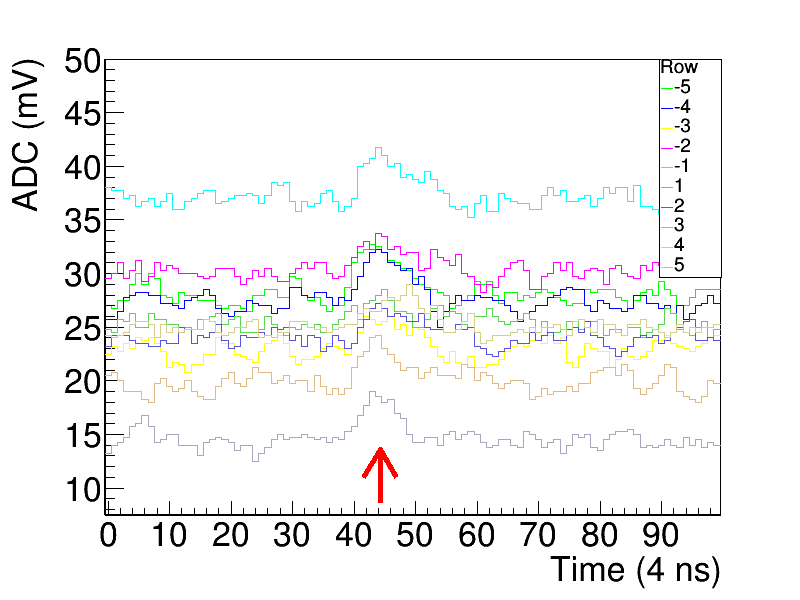
\includegraphics[width=0.5\textwidth]{pics/cosmicSignal.png}
  \caption{Cosmic ray signal passing vertically through all ten layers of crystals in the Ecal. Each crystal's signal is separated vertically in this plot by an offset (pedestal). The arrow indicates the approximate place in time that the cosmic signal passed through the detector.}
  \label{cosmicSignal}
\end{figure}	

As shown in Figure ~\ref{cosmicSignal}, each FADC channel has a unique pedestal value. The pedestal for each event was calculated as an average of the FADC counts in the first twenty bins of the time window. The integrated signal was used for the final calibration. By searching for a threshold crossing (thresholds were 2.5~mV in 2015 with splitters, 3.5~mV in 2016 after spliter removal) in the time window where cosmic events occurred, the signal was then fully integrated and the pedestal was subtracted. Geometric cuts are then applied to the data in offline analysis. Crystals having peaks over a certain threshold must have at least adjacent crystals located above and below with threshold crossing, but the crystals to the left and right must not cross threshold. These cuts ensure that the track passed as vertically as possible through the Ecal (reducing the variations of path length across each crystal). The integrated signals over many events in each crystal were fit. An individual crystal fit is shown in Figure ~\ref{cosmicFit}. 

\begin{figure}[H]
  \centering
      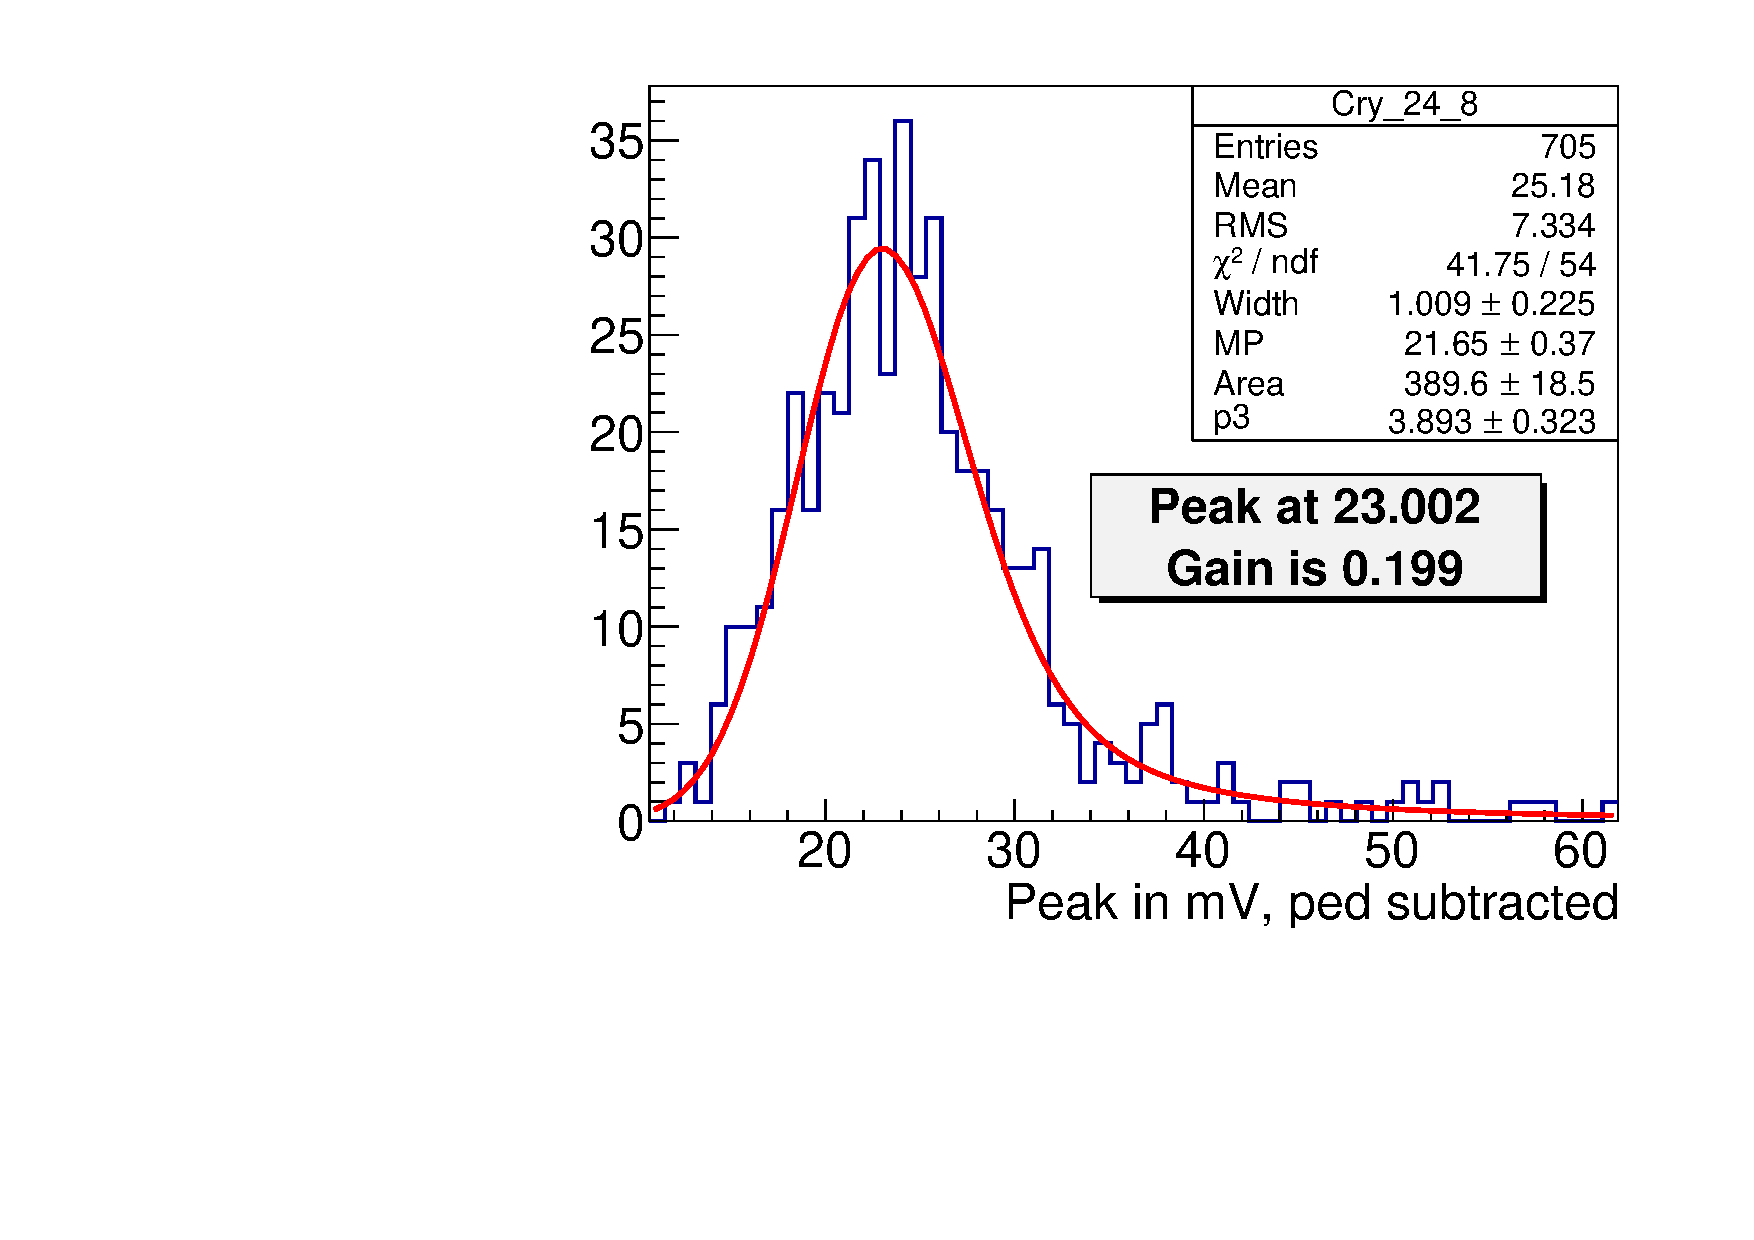
\includegraphics[width=0.5\textwidth]{pics/cosmicFitExample.pdf}
  \caption{Each cosmic signal was integrated and then fit using a Landau-Gaussian convolution. The peak was calculated numerically from this fit.}
  \label{cosmicFit}
\end{figure}

The fit shown in Figure ~\ref{cosmicFit} utilized a Landau-Gaussian convolution as the Landau part corresponds to the crystal's response to a particle's energy deposition as ionization energy loss, and the Gaussian part accounts for the statistical nature of the electronics shaping and readout. The peak of the fit is calculated numerically, and the initial conversion from units of FADC to energy (MeV) is obtained (called Gain factor). The unit conversion from units of mV to FADC is 1~V to 4096 FADC.\footnote{The 4096 FADC counts can be set to 1~V or 2~V, but for 2015 and 2016 running, the setting was 1~V. While this conversion is not explicitly stated in the reference\cite{CODA}, it comes from the 12~bit conversion which yields 4095 FADC.} Using the peak position for each crystal in units of FADC and by knowing the energy deposition of cosmic ray muons from simulation, the gain factor is calculated as shown in Equation ~\eqref{eq:gain}.

\begin{equation}
\label{eq:gain}
Gain = \dfrac{[MeV]}{[FADC]} 
\end{equation}
	 
After approximately 60 hours of cosmic data, the entire Ecal could be calibrated using cosmics, and the resultant gains for all channels is shown in Figures ~\ref{cosmicGain} and ~\ref{cosmicGain1D}.

\begin{figure}[H]
  \centering
      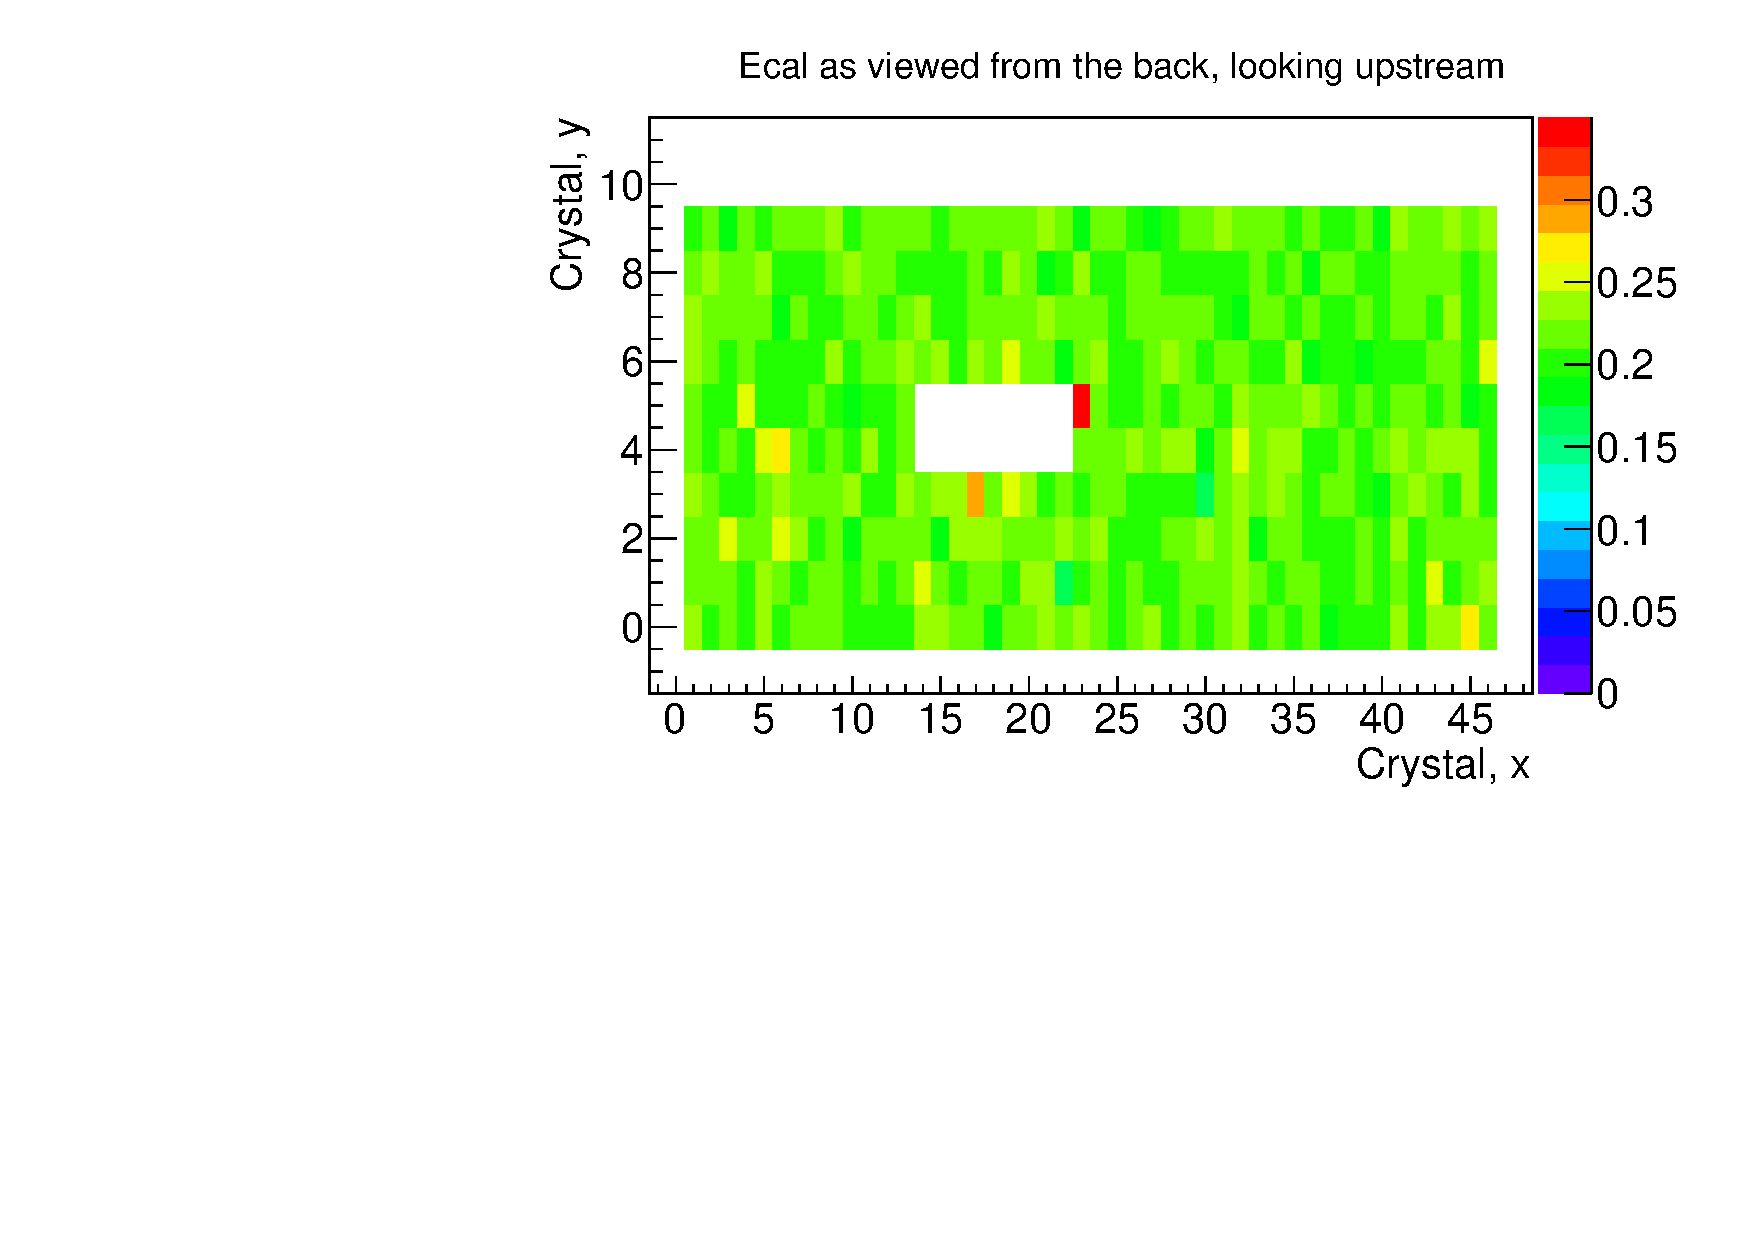
\includegraphics[width=0.48\textwidth]{pics/cosmicGains_2015.pdf}
  \caption{Resulting gain calibration using cosmics for all crystals.}
  \label{cosmicGain}
\end{figure}

\begin{figure}[H]
  \centering
      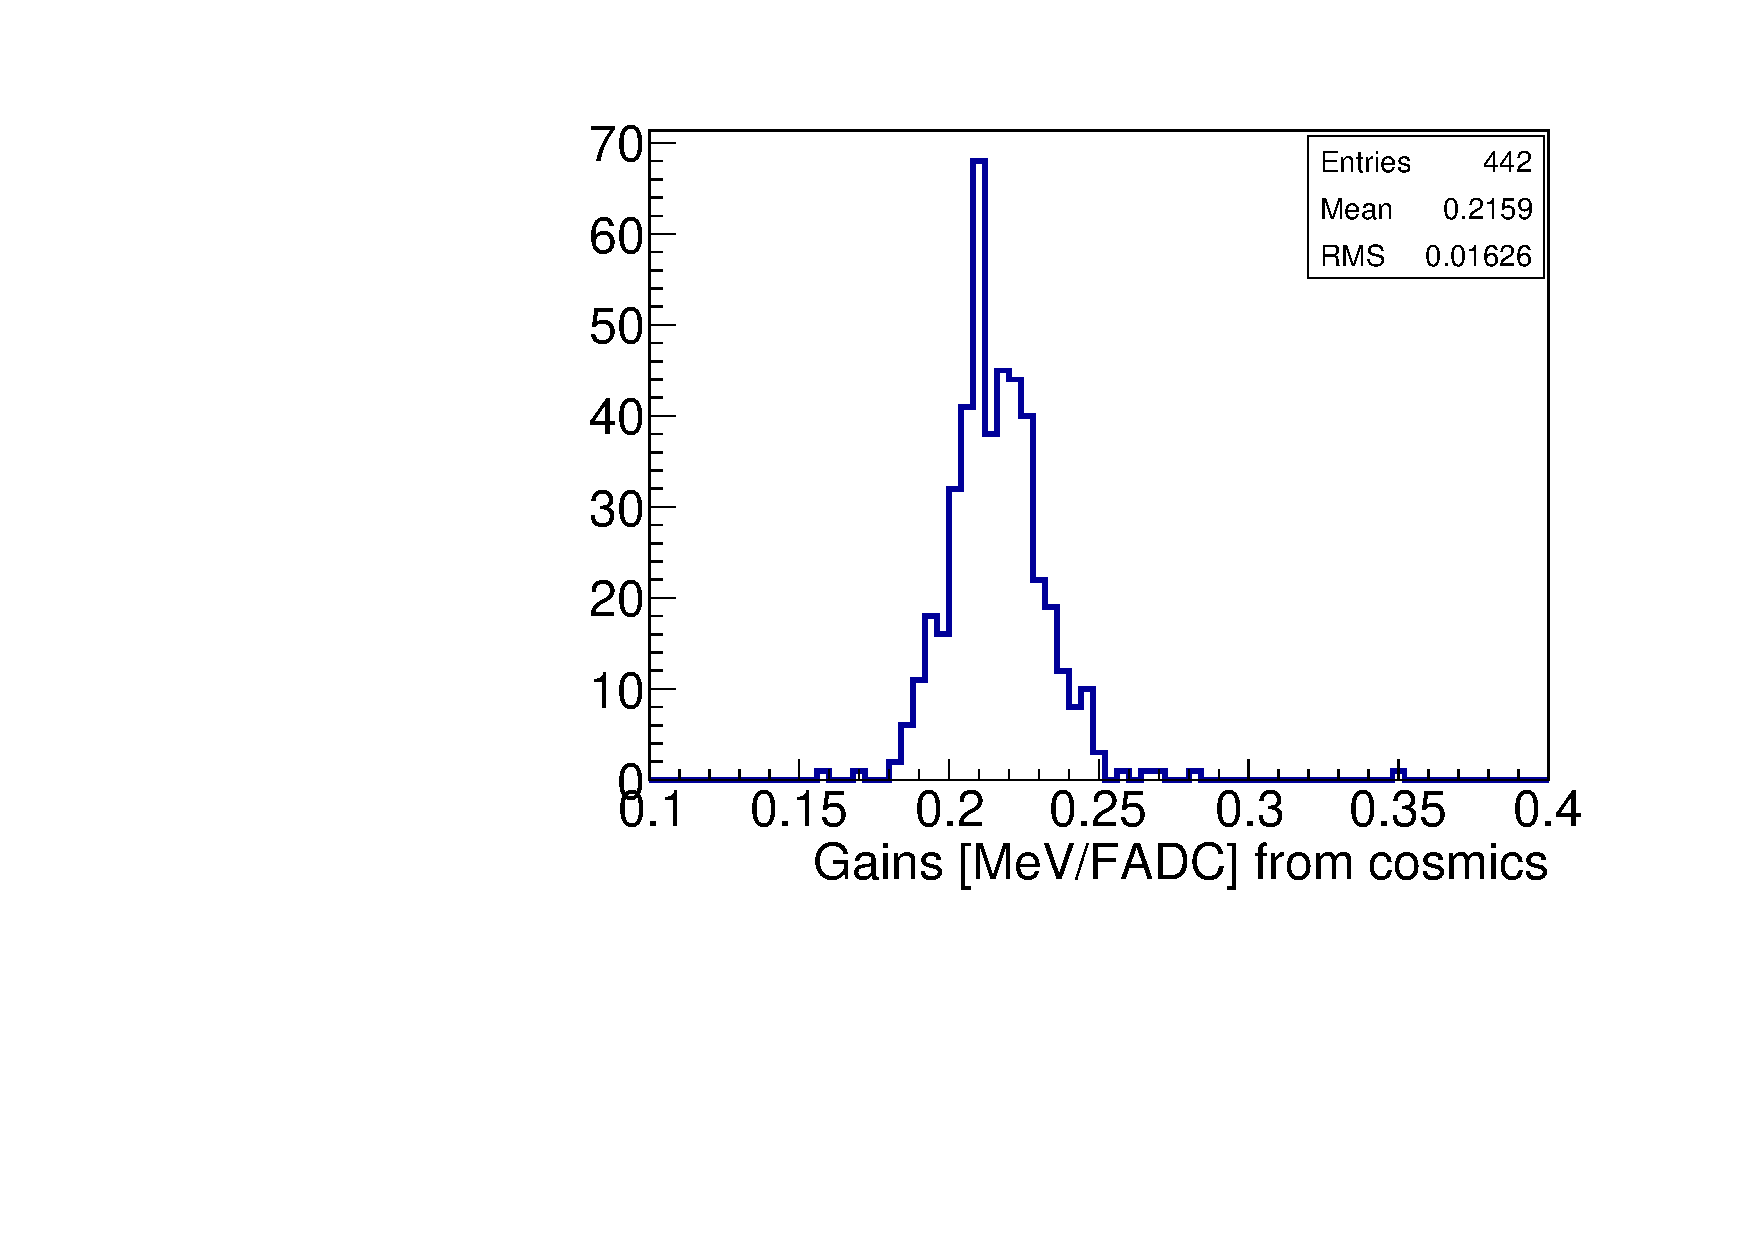
\includegraphics[width=0.5\textwidth]{pics/cosmicGainsMay15.pdf}
  \caption{Resulting gains using cosmics for all crystals.}
  \label{cosmicGain1D}
\end{figure}
	
The resultant gains from cosmics shown above is from the cosmic calibration performed in May 2015. This calibration was used as the basis for further calibrations of the data from 2015 running. 	
	
\subsection{Elastically-Scattered Electrons}
The cosmic calibration was sufficient for the initial data-taking with the electron beam.  The  electrons detected in the Ecal by elastic scattering from the target peak at the beam energy of approximately 1~GeV. Electromagnetic calorimeters collect a proportional amount of the energy deposited. In order to fully reconstruct all of the incident energy of the electron, one must apply sampling fraction corrections to the measured cluster energies. For this study, events were selected in which the energy of the seed hit in a cluster, or the hit with the highest energy, carried greater than 60\% of the cluster energy, the seed hit carried an energy greater than 450 MeV, and the cluster occurred within the timing window for a singles1-type trigger. The cluster energy was then associated with the seed hit crystal. The first step of the elastically-scattered electron calibration is studying the uncorrected cluster energy deposited in the Ecal from simulation. Simulation shows which regions of the calorimeter can accept elastically-scattered electrons. Certain regions of the Ecal are out of acceptance for this calibration due to geometric effects and detector configuration as shown in Figure ~\ref{fee_sim}. 
	
\begin{figure}[H]
  \centering
      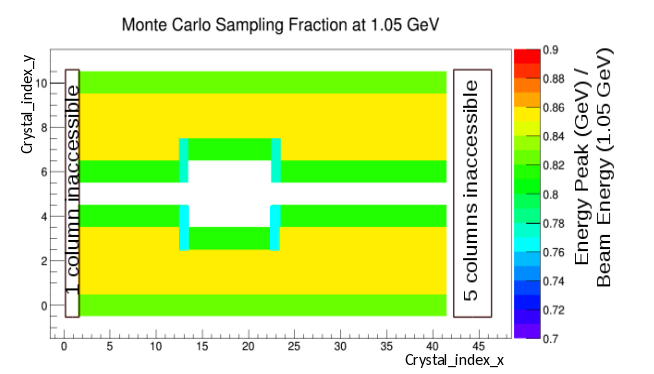
\includegraphics[width=0.5\textwidth]{pics/fee_acceptance.png}
  \caption{Sampling fraction of elastically-scattered electron clusters in the Ecal from simulation. Simulation shows certain regions of the calorimeter are inaccessible to elastically-scattered electrons at 1.05 GeV.}
  \label{fee_sim}
\end{figure}	
	
	The distribution of sampling fractions in Figure ~\ref{fee_sim} shows that we are unable to calibrate the first column of crystals on Beam Right and five columns of crystals on Beam Left using elastically-scattered electrons. The energy deposited in a crystal from data is compared to that found in Monte Carlo. An example fit to the energy distribution of elastic electrons from data when one particular crystal was the seed is shown in Figure ~\ref{feeExample}:
	
\begin{figure}[H]
  \centering
      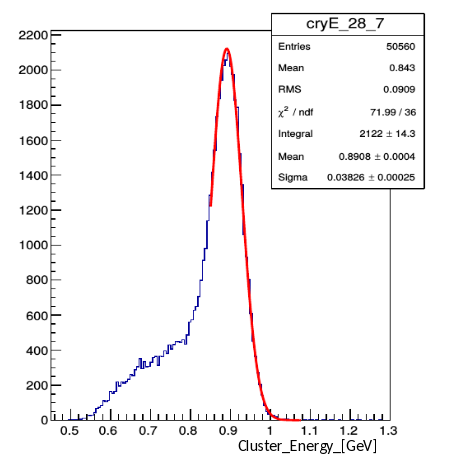
\includegraphics[width=0.5\textwidth]{pics/indifvidualfeefit.png}
  \caption{Asymmetric Gaussian fit to the elastic energy peak(uncorrected) when crystal index (+5,+2) was the seed hit.}
  \label{feeExample}
\end{figure} 	
	
The peak position obtained from fitting the cluster energy distribution with an asymmetric Gaussian as in Figure ~\ref{feeExample} is used to calculate an iteration factor, or a factor to be multiplied by the original gain value obtained from the cosmic calibration, in order to scale the energy up or down as needed to match simulation. The iteration factor is calculated for each crystal that has acceptance as the seed crystal for elastically-scattered electrons and then applied to the corresponding crystal's gain. Reconstruction is then performed on all events, and this fitting process is repeated until the iteration coefficient is within 1\% of the Monte Carlo peak position. An iteration coefficient is obtained from the fitted peaks as shown in Equation ~\eqref{eq:iterFactor}:
	
\begin{equation}
\label{eq:iterFactor}
C_i = \dfrac{MC_{peak}}{data_{peak}}
\end{equation}	
	
	Crystals that could not be calibrated using elastically-scattered electrons were assigned an iteration coefficient of 1. The iteration coefficients for each crystal during the first round of calibration are shown in in Figure ~\ref{feeiter1}. 	
	
\begin{figure}[H]
  \centering
      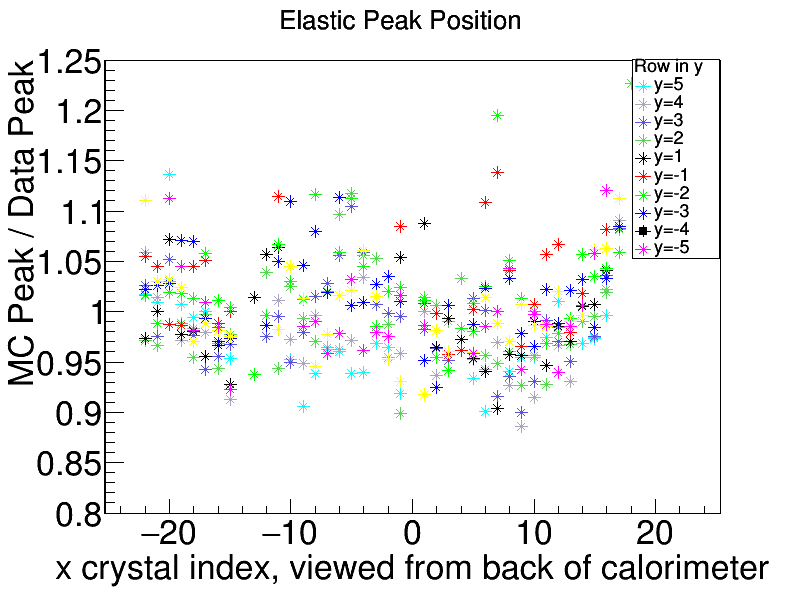
\includegraphics[width=0.5\textwidth]{pics/feeiter2.png}
  \caption{Ratio of elastic peak position in each crystal versus the peak position in each crystal as found in Monte Carlo before calibration.}
  \label{feeiter1}
\end{figure}	

From Figure ~\ref{feeiter1}, one can see that there is variation from crystal to crystal in the peak position with respect to its position as calculated from simulation. After completing two successive iterations of the elastically-scattered electron calibration, the 366 crystals that had geometric acceptance for elastically-scattered electrons were calibrated to within 1\% of the Monte Carlo cluster peak locations as shown in Figure ~\ref{feeiter3}.  

\begin{figure}[H]
  \centering
      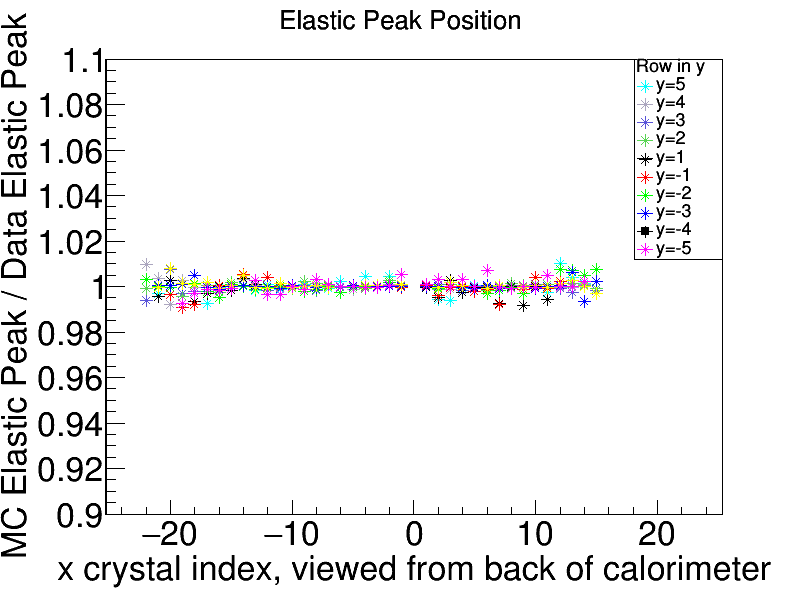
\includegraphics[width=0.5\textwidth]{pics/feeiter3.png}
  \caption{Ratio of elastic peak position in each crystal versus the peak position in each crystal as found in Monte Carlo after calibration.}
  \label{feeiter3}
\end{figure}

After completing the calibration procedure, the sampling fraction correction function found in simulation was applied to the measured cluster energies. A histogram containing all of the elastically-scattered electron clusters in the fiducial region Ecal (where seed hits are not on edge crystals) can be seen in Figure ~\ref{feeTotal}. 
	
\begin{figure}[H]
  \centering
      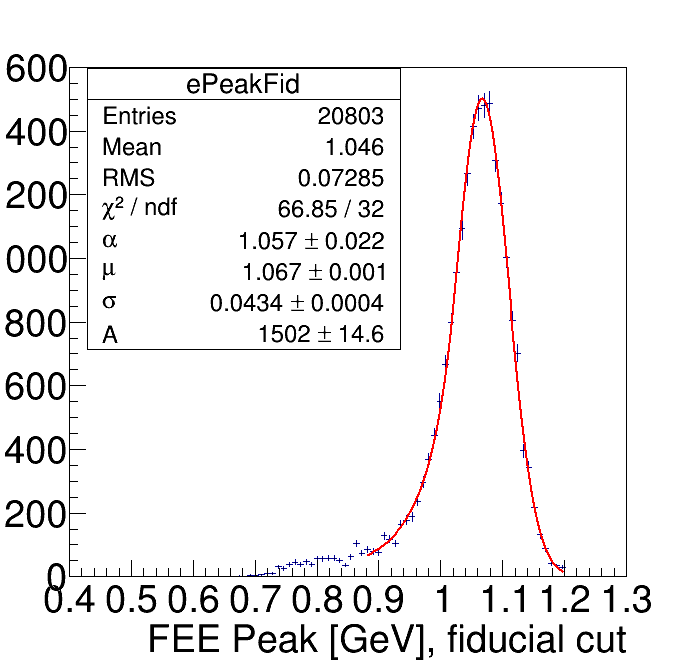
\includegraphics[width=0.5\textwidth]{pics/feerestotalX.png}
  \caption{Elastically-scattered electron peak as seen in the Ecal, after calibration.This plot utilizes a fiducial cut which excludes clusters with a seed hit in an edge crystal.}
  \label{feeTotal}
\end{figure} 
    
	The cluster energy spectrum in Figure ~\ref{feeTotal} is fit with a Crystal Ball Function which contains a Gaussian component and a power law low energy tail. The fit shown in Figure ~\ref{feeTotal} demonstrates that the Ecal has an energy resolution of 4\% in the fiducial region after calibration. Prior to calibration, this number was approximately 8\%. The final gains that were obtained from calibration are shown in Figures ~\ref{feegains} and ~\ref{feegains1D}. 
	
\begin{figure}[H]
  \centering
      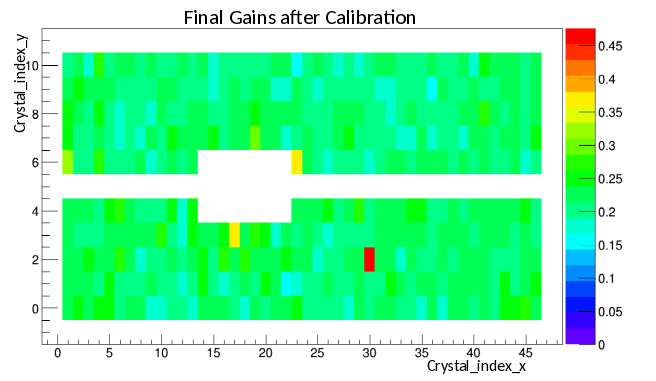
\includegraphics[width=0.5\textwidth]{pics/finalGains.png}
  \caption{The final gains are shown for all crystals after the elastic energy calibration. The crystals that were not calibrated using elastically-scattered electrons were calibrated from cosmics.}
  \label{feegains}
\end{figure}

\begin{figure}[H]
  \centering
      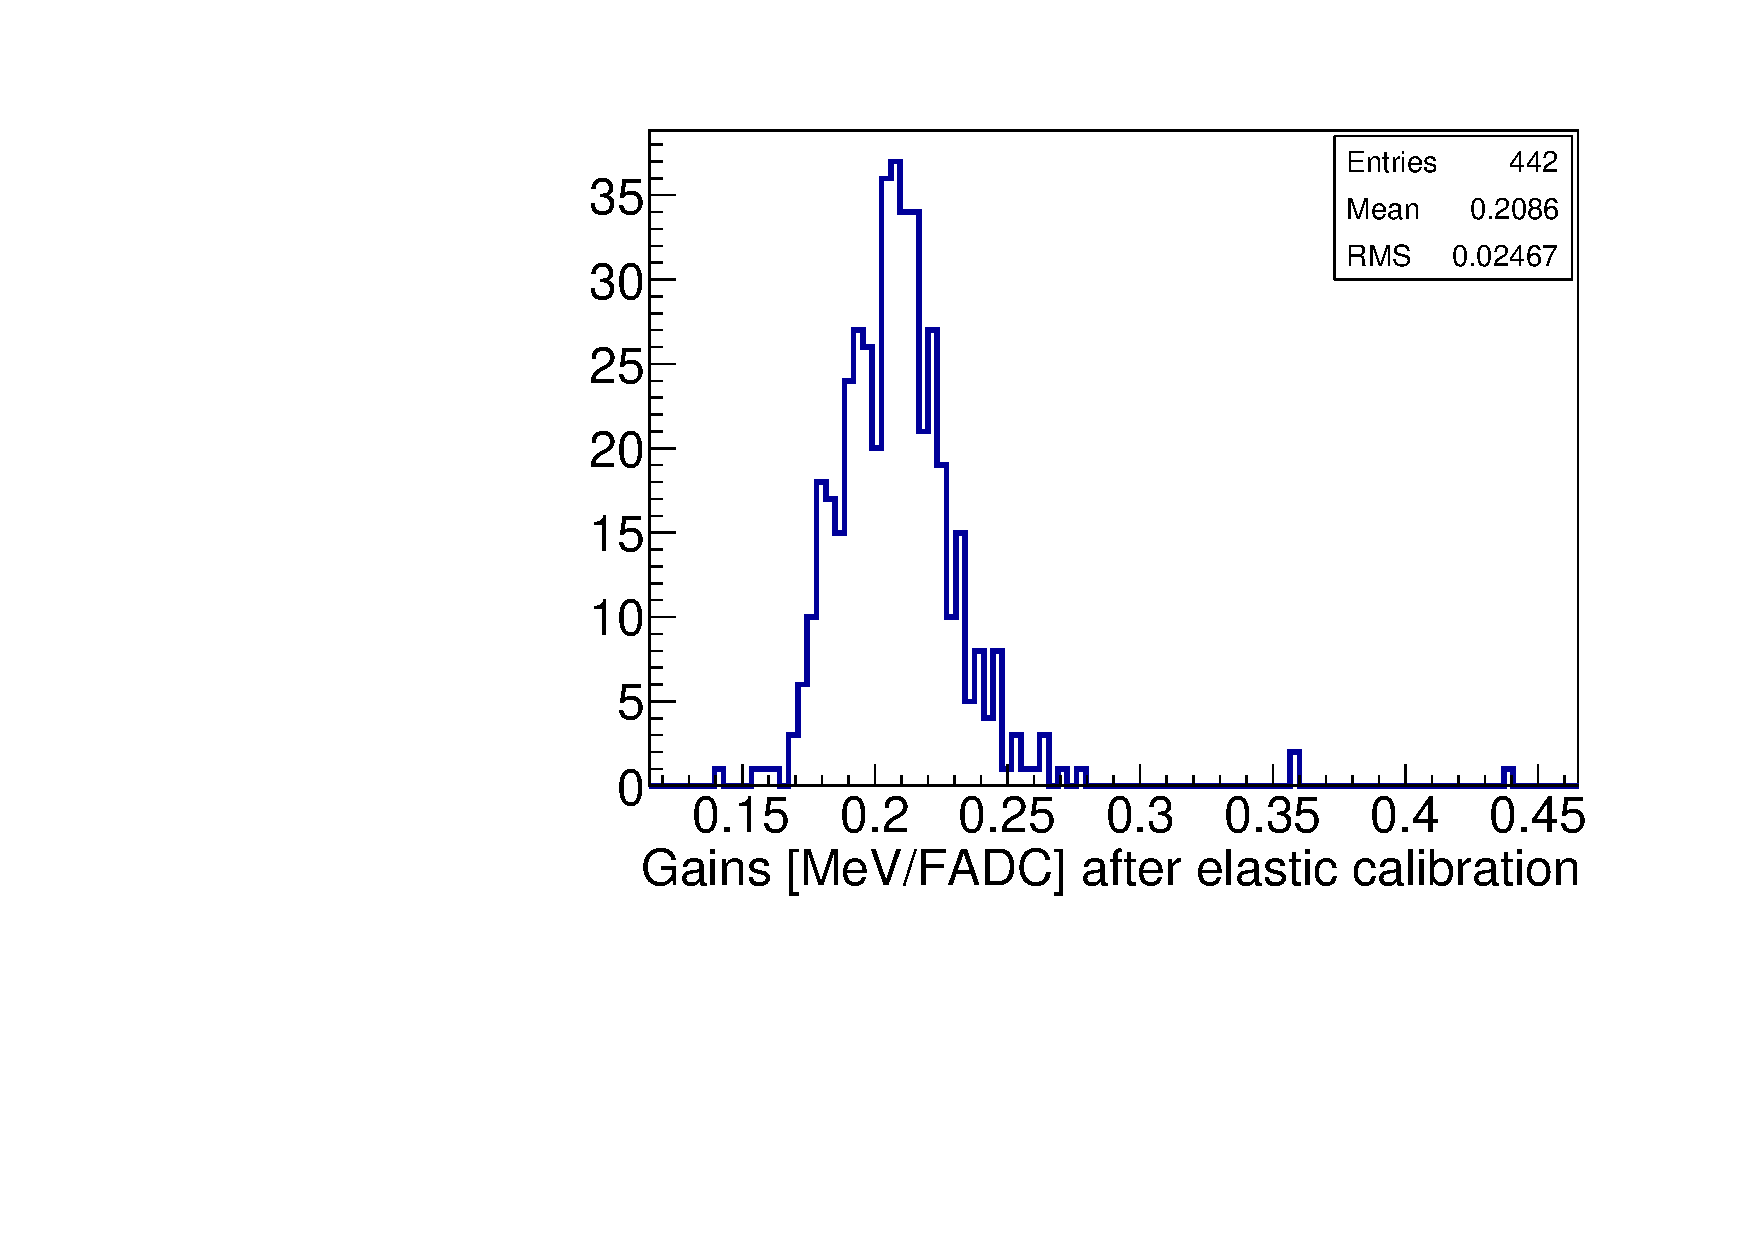
\includegraphics[width=0.5\textwidth]{pics/fee_2015gains.pdf}
  \caption{All gains after calibration of the 2015 data using cosmics and elastically-scattered electrons.}
  \label{feegains1D}
\end{figure}

Figures ~\ref{feegains} and ~\ref{feegains1D} contain the gains for all crystals, including those that were only calibrated with cosmics. The final gains of crystals that could be calibrated with elastically-scattered electrons were compared to their original cosmic gains as shown in Figure ~\ref{gaincomp}.
	
\begin{figure}[H]
  \centering
      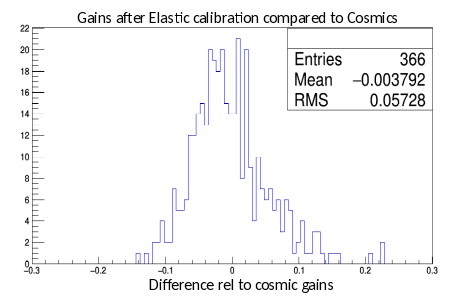
\includegraphics[width=0.5\textwidth]{pics/feeVcosmics.png}
  \caption{Comparison of gains obtained from the elastically-scattered electron calibration versus the gains obtained from the cosmic calibration. Only the 366 crystals that could be calibrated with elastics are compared.}
  \label{gaincomp}
\end{figure} 

The comparison of the gains shows that the cosmic calibration was roughly accurate within $\pm$10\%. Comparing the low energy and high energy calibrations as in Figure ~\ref{gaincomp} can tell us that the initial energies used in the cosmic calibration are roughly accurate, but it is limited in telling us anything about the linearity of the gain between these two points.  

\subsection{Wide-Angle Bremsstrahlung}
Wide Angle Bremsstrahlung (WAB) is an extremely useful physics process for  further energy characterization of the Ecal. The primary physics trigger looking for two cluster events recorded a very high yield of WAB particles which is composed of a photon and an electron. The WAB spectrum is shown in events with two clusters in Figure ~\ref{WABband} as events occurring along the diagonal black line where the energy sum of the two particles is approximately equal to the beam energy (uncorrected).

\begin{figure}[H]
  \centering
      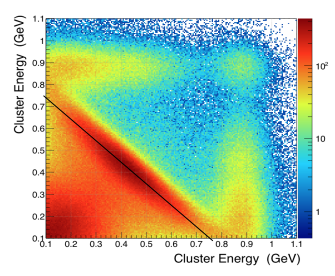
\includegraphics[width=0.5\textwidth]{pics/twoclusterenergies.png}
  \caption{Uncorrecter cluster energies for two cluster events. The diagonal band, where the two clusters sum to the beam energy, contains WAB events.}
  \label{WABband}
\end{figure} 

Initial studies after the elastic energy calibration showed that the energy sum of two particles in exclusive events was   lower than beam energy which means that the Monte Carlo sampling fraction correction functions in the mid-beam energy region needed refining. By studying events from wide angle bremsstrahlung, the necessary adjustments have been understood. WAB events are identified by track-matched electrons using SVT momentum information and unmatched photon clusters. 
	A few constraints were necessary in order to construct the analysis for studying the sampling fraction corrections in data across a range of energies. The first constraint is that the energy sum of the two particles, sampling fraction corrected, must be equal to the energy of the beam:
\begin{equation}
\label{eq:particlesum}
\dfrac{E_{e-}}{SF_{e-}(E_{e-})} + \dfrac{E_{\gamma}}{SF_{\gamma}(E_{\gamma})} = E_{i}
\end{equation}		
	
In Equations ~\eqref{eq:particlesum} and ~\eqref{eq:sfratio}, $SF$ refers to the sampling fraction correction functions described by Equation ~\ref{eq:samplingfraction}. The second constraint is that the relationships between the electron and photon sampling fractions found in Monte Carlo must be preserved by what is found in data:
\begin{equation}
\label{eq:sfratio}
\dfrac{SF_{e-,data}(E_{e-})}{SF_{\gamma,data}(E_{\gamma})} = \dfrac{SF_{e-,MC}(E_{e-})}{SF_{\gamma,MC}(E_{\gamma})}
\end{equation}

By maintaining the two assumptions in Equations ~\eqref{eq:particlesum} and ~\eqref{eq:sfratio}, a chi-squared minimization can yield the optimal adjustments to the sampling fraction for mid-range energies. This is shown in Equation ~\ref{eq:chisquare}.
\begin{equation}
\label{eq:chisquare}
\chi^2 = \Sigma_i \dfrac{(E_{beam}-E_{i})^2}{\sigma_{e-}^2(E_{e-})+\sigma_{\gamma}^2(E_{\gamma})}
\end{equation}

For each event, the energy sum of the two corrected clusters, $E_i$, is calculated as described by Equation ~\eqref{eq:particlesum}. The end result is an adjustment made to the parameters in the sampling fraction correction functions. Additionally, elastically-scattered electron events were incorporated in order to ensure that the peak for a single energy electron is still at the beam energy. Adjustments to the sampling fraction parameters yielded new sampling fraction correction functions. The ratio of the new to old sampling fraction correction functions is shown in Figure ~\ref{sfchange} for electrons:
\begin{figure}[H]
  \centering
      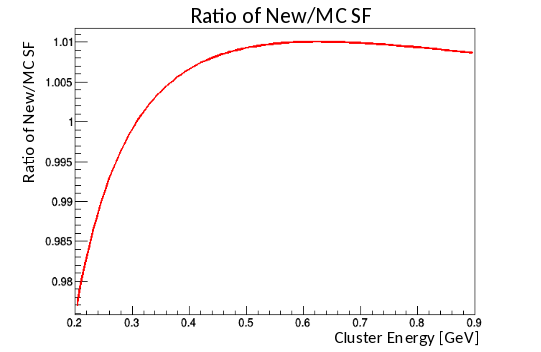
\includegraphics[width=0.5\textwidth]{pics/sfchangewab.png}
  \caption{Change relative to the Monte Carlo-simulated sampling fraction as found by studying the WAB energy spectrum.}
  \label{sfchange}
\end{figure} 

After incorporating these updated sampling fraction correction functions as found in data, the energy resolution from data could be found as a function of particle energy. In Figure ~\ref{wabsum}, one can observe the energy sum of the two WAB particles when the electron and photon energies differ by less than 50 MeV. 
\begin{figure}[H]
  \centering
      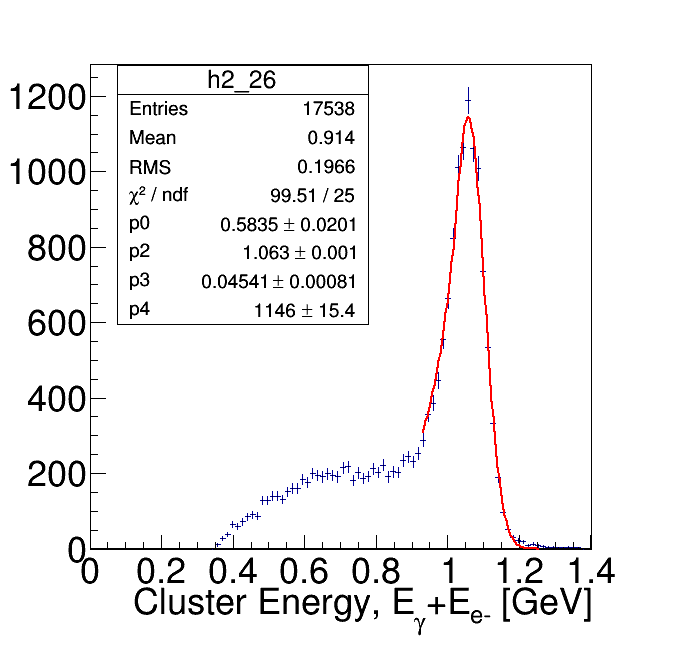
\includegraphics[width=0.5\textwidth]{pics/wabsum.png}
  \caption{The energy sum of two particles peaks at the same location as a single elastically-scattered electron.}
  \label{wabsum}
\end{figure}

From studying the energy sum of various energy combinations of WAB particles, the full energy resolution for electrons was able to be measured. 

%------------------------------------------------

\section{Results}
\subsection{Fiducial Resolution}
The timing offsets and energy calibration were incorporated into the cluster-building process during offline event reconstruction. The elastically-scattered electron calibration provided the most clear point in understanding the measured energy resolution in the Ecal at the beam energy. WAB events were used to identify the energy resolution at energies other than beam energy. The energy resolution of electrons could be studied both as a function of energy and as a function of position relative to the edges of the Ecal (energy resolution deteriorates rapidly in edge crystals). The resulting energy resolution as a function of energy is shown in Figure ~\ref{eres}. 
\begin{figure}[H]
  \centering
      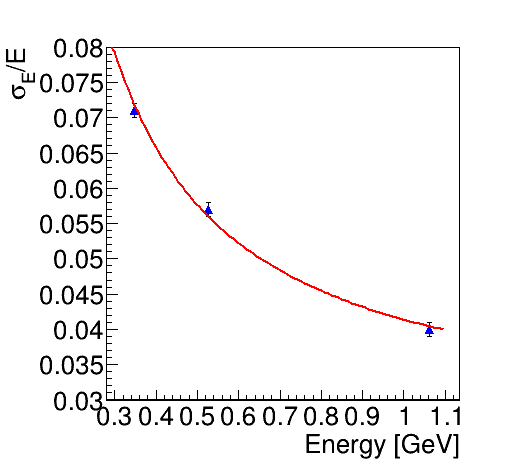
\includegraphics[width=0.5\textwidth]{pics/resolution.png}
  \caption{Energy resolution in the Ecal as found in data. The fit is described by the general energy resolution function and is shown in Equation ~\ref{eq:enres}.}
  \label{eres}
\end{figure}

In order to study the energy resolution in the fiducial region of the Ecal, all electrons were matched to tracks, and the track position at the Ecal was used to determine the electron's distance from the beam gap edge. For elastically-scattered electrons, only one electron is used. In the case of WAB, the photon is not matched to a track. By requiring the photon to be at least 10~mm from the Ecal edges (in the fiducial region), the cluster energy for the photon is generally reliable. The elastically-scattered electron established the point for the energy resolution at the highest possible detected energy in Figure ~\ref{eres}.\\
\indent The middle energy point at approximately 0.5 GeV was obtained by selecting WAB events where the energy difference between the two particles was less than 100 MeV. By fitting the energy sum of the two particles, as reported by the Ecal, the resolution of the electron was able to be found  after subtracting the contribution from the photon. By selecting only events where both particles are in the fiducial region, the energy resolution of the sum could be divided by $\sqrt{2}$ assuming that the resolution of the electron and photon are the same due to the energy difference being quite small. This resolution could be extracted by using Equation ~\eqref{eq:resExtract}.


\begin{equation}
\label{eq:resExtract}
\sigma_{E_{1}+E_{2}}^{2} = \sigma_{e-}^2(E_1)+\sigma_{\gamma}^2(E_2)
\end{equation}

This same procedure was used to find the resolution for highly asymmetric energy clusters. The lowest energy point used to study resolution is at approximately 350~MeV. While varying the energy resolution curve derived from Monte Carlo and characterizing the data points at the full and half beam energy in data, it was observed that the resolution at 0.7~GeV was relatively unchanged. When subtracting the 0.7~GeV resolution from the resolution of the energy sum of the 350 and 700~MeV WAB particles, the resultant resolution for the 350 MeV particle was approximately 7.1$\%$. This was consistent with measuring the resolution of the peak of 350~MeV particles when selecting 700 MeV photons in the fiducial region.\\
\indent The experimentally-obtained energy resolution agrees well with Monte Carlo but generally yields a slightly larger energy resolution for all energies (on the order of about 15$\%$). Understanding the energy resolution, precisely, is critical if one is to combine the measurements obtained between the SVT and the Ecal in order to improve the invariant mass resolution for a heavy photon search. The fit to the energy resolution in the data is shown in Equation ~\ref{eq:enres}.
\begin{equation}
\label{eq:enres}
\dfrac{\sigma_E}{E}(\%)=\dfrac{1.62}{E}\oplus \dfrac{2.87}{\sqrt{E}} \oplus 2.5
\end{equation}
 
Equation ~\eqref{eq:enres} can be compared to the energy resolution as derived from Monte Carlo ~\cite{Garcon} in Equation ~\eqref{eq:MCenres}:
\begin{equation}
\label{eq:MCenres}
\dfrac{\sigma_E}{E}(\%)=\dfrac{1.65}{E}\oplus \dfrac{2.62}{\sqrt{E}} \oplus 1.8
\end{equation}
 
 In Equations ~\eqref{eq:enres} and ~\eqref{eq:MCenres}, the first term is generally attributed to the noise from the pre-amplifiers and is consistent between data and Monte Carlo. The second term is related to the statistical fluctuations of the shower containment and the APD gain. The second term is slightly larger in data than that derived from Monte Carlo but is consistent. The third term contains both the energy leakage out the back of the Ecal as well as the crystal-to-crystal inter-calibration error. This term is significantly higher in data than that derived from Monte Carlo, but this term is consistent with what was derived using the same crystals for the CLAS Inner Calorimeter ~\cite{FX}.
 
\subsection{Edge Effects} 
In order to study the energy resolution effects at the edges of the Ecal, events from both WAB and elastically-scattered electrons were used. Once resolution  in the fiducial region of the Ecal was extracted, one could find the energy resolution for all electrons going to the edge of the Ecal. This was accomplished at various energies by studying elastically-scattered electrons and WAB events (looking at the energy sum of the two particles) with track-matched electrons and photons. By requiring the photons to be within the fiducial region of the Ecal, the photon's contribution to the resolution of the energy sum could be subtracted as in Equation ~\eqref{eq:resExtract}. The peak position and width of the energy sum distribution for two nearly-equal energy particles is shown in ~\ref{wabHalf} where the electron's position is used.

\end{multicols}

\begin{figure}[H]
  \centering
      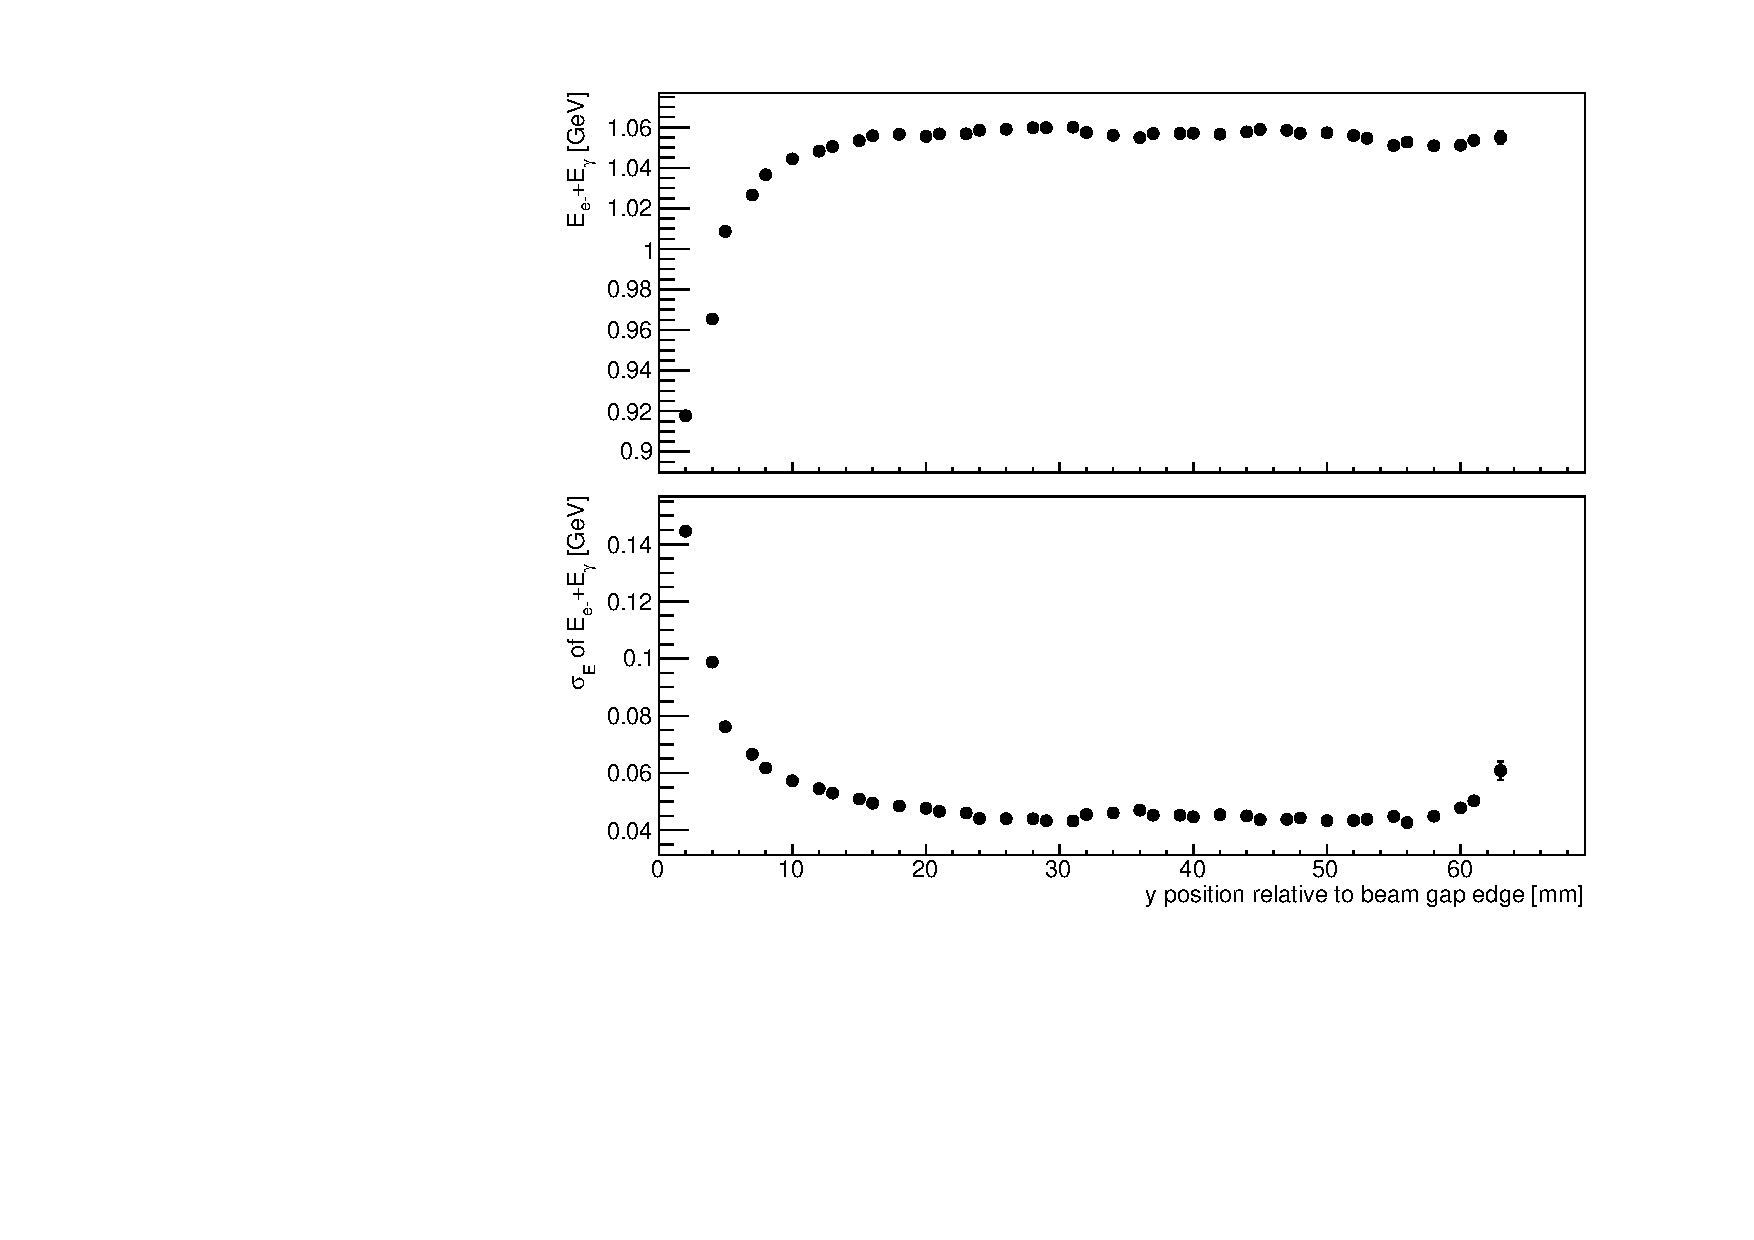
\includegraphics[width=1.0\textwidth]{pics/WAB_sumHalf.pdf}
  \caption{By studying two nearly equal energy particles in WAB, the energy sum can be plotted for various vertical positions of the electron across the Ecal. The position here is given from the track-matched electron and using the projected track position of the electron at the Ecal. The width of the sum of those distributions is plotted in the lower plot. }
  \label{wabHalf}
\end{figure}
  
\begin{multicols}{2} 

By using the extracted resolution of the electron as full beam energy, half beam energy, and ~350 MeV, the energy resolution could be characterized as a function of position relative to the beam gap edge of the Ecal. It was found that the second parameter of the energy resolution function as described by Equation ~\eqref{eq:enres}, now denoted as $B/\sqrt{E}$, is strongly correlated to the position in the Ecal. By fixing the other two terms to the values in the fiducial region, the $B$ parameter was studied with respect to position within the Ecal. For each position in y relative to the inner beam gap edge, the energy resolution function could be fit with the free parameter as shown for a single slice in y in Figure ~\ref{sliceY}.

\begin{figure}[H]
  \centering
      \includegraphics[width=0.45\textwidth]{pics/examplebparfit3.pdf}
  \caption{This shows an example fit for the second parameter of the energy resolution function for a specific slice in a y relative position to the inner beam gap edge.}
  \label{sliceY}
\end{figure}

The final relationship between the $B$ parameter and position in the Ecal is shown in Figure ~\ref{BparRes}.
   
 \begin{figure}[H]
  \centering
      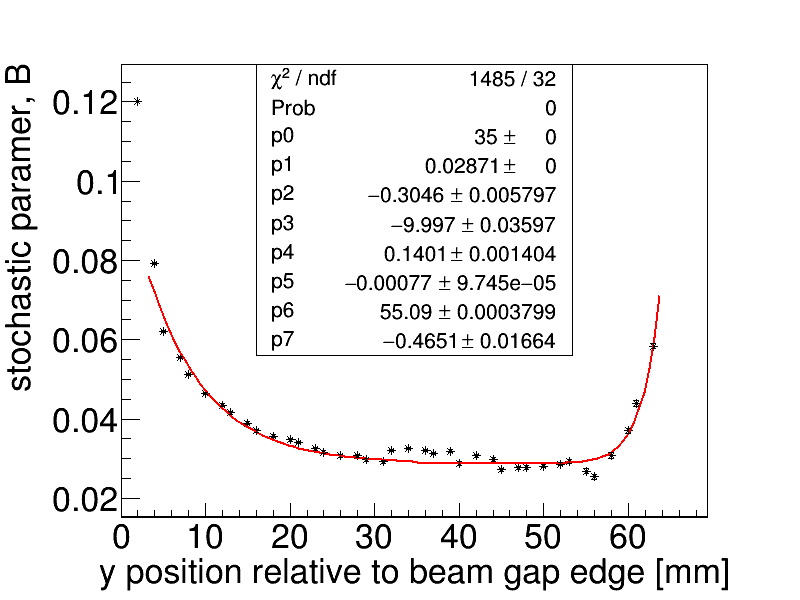
\includegraphics[width=0.5\textwidth]{pics/money.png}
  \caption{The change in the stochastic parameter (corresponding to $1/\sqrt{E}$ term) of the energy resolution description as a function of its position relative to the beamgap edge of the Ecal. The fit is described by Equation ~\ref{eq:finalRes} such that the value is matched in the central, fiducial region of the Ecal.}
  \label{BparRes}
\end{figure}
 
 
 The final function for the energy resolution in the Ecal is now read as both a function of energy and y position relative to the inner beam gap edge as shown in Equation ~\eqref{eq:finalRes}.
 
 \begin{equation}
\begin{split}
\label{eq:finalRes}
\dfrac{\sigma_E}{E}(\%)=\dfrac{1.62}{E}\oplus \dfrac{B(y)}{\sqrt{E}} \oplus 2.5 \\
B(y<p_0) = p_1-p_2 e^{-(y-p_3)p_4}\\
B(y>p_0) = p_1-p_5 e^{-(y-p_6)p_7}
\end{split}
\end{equation}

The energy distribution in the Ecal is asymmetric, having a low energy tail. The resolution parameterizations are generally reliable down to 6.5~mm from the edge of the crystal (center of the crystal face), but the energy resolution is deteriorating rapidly after 8-10~mm to the edge of the crystal. 
  


%------------------------------------------------

\section{Conclusions}

After a successful experimental run in the spring of 2015, all elements of the HPS detectors and beamline were commissioned. Calibrations were completed and cross-checked using various physics processes that enabled the full understanding of the energy resolution of the Ecal. Preliminary studies show that the Ecal provides a resolution comparable to that of the SVT momentum resolution and could be combined to improve the overall measurement of the invariant mass for certain ranges of masses that HPS searches in for the heavy photon. From the spring 2015 running, HPS searches for the heavy photon at strong and weak couplings using a blind analysis procedure. This summary details the procedures used to calibrate the Ecal.  

%----------------------------------------------------------------------------------------
%	REFERENCE LIST
%----------------------------------------------------------------------------------------

\begin{thebibliography}{99} % Bibliography - this is intentionally simple in this template

\bibitem{Baltzell} N. Baltzell,\href{https://confluence.slac.stanford.edu/download/attachments/192191938/3PoleAna.pdf?version=1&modificationDate=1434062944000&api=v2}
HPS Note 2015-010.

\bibitem{Garcon} H. Szumila-Vance, M. Garcon,\href{https://misportal.jlab.org/mis/physics/hps_notes/viewFile.cfm/2014-001.pdf?documentId=1}
HPS Note 2014-001.

\bibitem{FX} F.X. Girod, M. Garcon,
\href{https://misportal.jlab.org/ul/Physics/Hall-B/clas/viewFile.cfm/2005-001.pdf?documentId=6}
CLAS Note 2005-001.

\bibitem{Kazimi} R. Kazimi, Simultaneous Four-Hall Operation for 12 GeV CEBAF, Proceedings of IPAC 2013, Shanghai, China.

\bibitem{pdg}   K.~A.~Olive {\it et al.} [Particle Data Group Collaboration], 
\href{http://pdg.lbl.gov/2009/AtomicNuclearProperties/MUON_ELOSS_TABLES/muonloss_301.ps}
Chin.\ Phys.\ C {\bf 38}, 090001 (2014).

\bibitem{Szumila} H. Szumila-Vance,\href{https://misportal.jlab.org/mis/physics/hps_notes/viewFile.cfm/2015-011.pdf?documentId=13}
HPS Note 2015-011.

\bibitem{CODA} E. Jastrzembski, H. Dong,
\href{https://coda.jlab.org/drupal/system/files/pdfs/HardwareManual/fADC250/FADC250%20data%20format%20V23.pdf}
Summary of FADC250 Operating Modes.


\end{thebibliography}

%----------------------------------------------------------------------------------------

\end{multicols}

\end{document}
